\documentclass[conference,compsoc,final,a4paper]{IEEEtran}
\usepackage[utf8]{inputenx}

%% Bitte legen Sie hier den Titel und den Autor der Arbeit fest
\newcommand{\autoren}[0]{Anton Bracke, Jannis Seefeld, Domenic Gosein, Maximilian Kürschner, Jan Mayer}
\newcommand{\dokumententitel}[0]{Development of an Autonomous Robot for Detecting and Collecting Objects}

% Hie muss normalerweise nichts angepasst werden
\usepackage[pdftex]{graphicx}
\graphicspath{{img/}}
\DeclareGraphicsExtensions{.pdf,.jpeg,.jpg,.png}
\usepackage[cmex10]{amsmath}
\usepackage{algorithmic}
\usepackage{array}
\usepackage{dblfloatfix}
\usepackage{url}
\usepackage[autostyle=true,english=american]{csquotes}
\usepackage[backend=biber,
            sorting=none,   % Keine Sortierung
            doi=true,       % DOI anzeigen
            isbn=false,     % ISBN nicht anzeigen
            url=true,       % URLs anzeigen
            maxnames=6,     % Ab 6 Autoren et al. verwenden
            minnames=1,     % und nur den ersten Autor angeben
            style=ieee,]{biblatex}
\usepackage{booktabs}
\usepackage{xcolor}
\usepackage{listings}             % Source Code listings
\usepackage[printonlyused]{acronym}
\usepackage{fancyvrb}
\usepackage{tocloft} % Schönere Inhaltsverzeichnisse

\usepackage[main=english, ngerman]{babel} % Englische Sprachunterstützung

\usepackage{tabularx}             % Spezielle Tabellen
\usepackage{svg}

% Farben definieren
\definecolor{linkblue}{RGB}{0, 0, 100}
\definecolor{linkblack}{RGB}{0, 0, 0}
\definecolor{darkgreen}{RGB}{14, 144, 102}
\definecolor{darkblue}{RGB}{0,0,168}
\definecolor{darkred}{RGB}{128,0,0}
\definecolor{comment}{RGB}{63, 127, 95}
\definecolor{javadoccomment}{RGB}{63, 95, 191}
\definecolor{keyword}{RGB}{108, 0, 67}
\definecolor{type}{RGB}{0, 0, 0}
\definecolor{method}{RGB}{0, 0, 0}
\definecolor{variable}{RGB}{0, 0, 0}
\definecolor{literal}{RGB}{31,0, 255}
\definecolor{operator}{RGB}{0, 0, 0}

\usepackage[
      unicode=true,
      hypertexnames=false,
      colorlinks=true,
      colorlinks=false,
      linkcolor=darkblue,
      citecolor=darkblue,
      urlcolor=darkblue,
      pdftex
   ]{hyperref}
%	 \PrerenderUnicode{ü}


% Einstellungen für Quelltexte
\lstset{
    xleftmargin=0.1cm,
    basicstyle=\scriptsize\ttfamily,
    keywordstyle=\color{keyword},
    identifierstyle=\color{variable},
    commentstyle=\color{comment},
    stringstyle=\color{literal},
    tabsize=2,
    lineskip={2pt},
    columns=flexible,
    inputencoding=utf8,
    captionpos=b,
    breakautoindent=true,
    breakindent=2em,
    breaklines=true,
    prebreak=,
    postbreak=,
    numbers=none,
    numberstyle=\tiny,
    showspaces=false,      % Keine Leerzeichensymbole
    showtabs=false,        % Keine Tabsymbole
    showstringspaces=false,% Leerzeichen in Strings
    morecomment=[s][\color{javadoccomment}]{/**}{*/},
    literate={Ö}{{\"O}}1 {Ä}{{\"A}}1 {Ü}{{\"U}}1 {ß}{{\ss}}2 {ü}{{\"u}}1 {ä}{{\"a}}1 {ö}{{\"o}}1
}

\hypersetup{
    pdftitle={\dokumententitel},
    pdfauthor={\autoren},
    pdfdisplaydoctitle=true,
    hidelinks
}

% Makros für typographisch korrekte Abkürzungen
\newcommand{\zb}[0]{z.\,B.}
\newcommand{\dahe}[0]{d.\,h.}
\newcommand{\ua}[0]{u.\,a.}

% Wo liegt Sourcecode?
\newcommand{\srcloc}{src/}

% Literatur einbinden
\addbibresource{literatur.bib}
 % Weitere Einstellungen aus einer anderen Datei lesen
\addbibresource{literatur.bib}   % BibLaTeX-Datei mit Literaturquellen einbinden

\begin{document}

% Titel des Dokuments
\title{\dokumententitel}

% Namen der Autoren
\author{
  \IEEEauthorblockN{\autoren}
  \IEEEauthorblockA{
    University of Applied Sciences Mannheim\\
    Department of Computer Science\\
    Paul-Wittsack-Str. 10,
    68163 Mannheim
    }
}

% Titel erzeugen
\maketitle
\thispagestyle{plain}
\pagestyle{plain}

% Eigentliches Dokument beginnt hier
% ----------------------------------------------------------------------------------------------------------

% Kurze Zusammenfassung des Dokuments
\begin{abstract}
Autonomous robots already have a broad spectrum of practical applications like autonomous delivery vehicles, warehouse, or service robots. The technology has also found its way into cars and is used for autonomous driving. As the technology behind it becomes more applicable, the question is what can a minimal autonomous robot setup look like and how does it work? This paper aims to answer that question by building a prototype capable of navigating toward objects with just one front camera, using the Robot Operating System (ROS) to control the robot and You Only Look Once (YOLO) for object detection. The paper describes different approaches to navigation and object detection and their challenges. It also goes into performance differences between YOLOv4 and YOLOv5. The outcome shows that it is possible to build such a minimal setup and that the best combination is a remote computer, which runs the object detection and sends commands to the robot for navigation. It also shows that YOLOv5 is much faster and more precise than YOLOv4. The biggest challenge however remains with the computing and network performance. Even though YOLO is very resource-saving and fast, the results indicate that more computing power and network throughput would lead to more fluid navigation. The robot is a semester project conducted as part of the course Autonomous Mobile Robots at the University of Applied Sciences Mannheim.

\noindent
\textit{Keywords: yolo, yolov4, yolov5, robot, autonomous robot, ros, turtlebot, turtlebot3 burger, object detection}
\end{abstract}

% Inhaltsverzeichnis erzeugen
{\small\tableofcontents}

\section{Introduction}

According to the Cambridge Dictionary, a robot is \enquote{a machine controlled by a computer that is used to perform jobs automatically} \autocite{dict-cambridge}. In the past years, the performance of those computers has increased while the size has decreased drastically. This recent development allows us to make use of some fascinating technologies like object recognition through neural nets. Object recognition or detection is part of computer vision and tries to simulate human vision through computational models. This technology can be used to build autonomous systems like cars or robots.

For this project, a pre-configured robot setup called Turtlebot Burger is used, which is a standard ROS-based robot platform \autocite{emanual-turtlebot3-ov}. The Robot Operating System (ROS) consists of a set of libraries and tools for building and running robots \autocite{ros-technical-overview}. The robot is additionally equipped with a camera for object detection and a fork to pick up detected objects along the way. YOLOv5 is used for object detection on the robot. It is a pre-trained neural net that only has to look at an image once to determine the objects inside it and thus is really fast and reliable \autocite{ultralytics}.

A containerized setup and code reload mechanism allowed for new ideas to be implemented and tested immediately on the running system.

The goal of this project is to see how good object recognition works with a minimal setup, resources, and a short amount of time to build. The scope of the project is purposely restricted to make use of only one front camera and avoid the usage of additional third-person cameras or sensors to show the great possibilities of such a minimal setup.

The test object is a tennis ball, which the robot should detect, collect and transport to a goal (object) of choice --- in this case a bottle. The paper starts by explaining the different components, technical setup, and navigation and the second half covers object detection.
\section{Basics}

This section describes the necessary basics for the hardware used in this project, as well as the operating system and the architecture behind the object detection.

\subsection{Robot Operating System (ROS)}
The Robot Operating System (ROS) is an open-source robotics meta-operating system for robots and as such provides hardware abstraction, low-level device control, message-passing between processes, and package management as well as tools and libraries for writing and running code across several computers \autocite{ros-intro}.

ROS consists of three concept levels, the file system level, the computation graph level, and the community level. The file system level covers things such as packages and the community level connects community members through different distributions and repositories. At the center is the computational graph, which is the peer-to-peer network for ROS processes consisting of nodes, master, parameter server, messages, services, topics, and bags. Nodes are processes that perform the computation, they communicate with each other by sending messages. Messages are subscribed to and published by topics. At the center the master takes care of registration and lookup, so nodes can find each other and exchange information --- as the below image shows \autocite{ros-concepts}.

\begin{figure}[!ht]
\centering
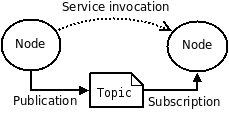
\includegraphics[width=4.5cm]{images/basics/ROS_basic_concepts.png}
\caption{ROS Basic Concepts \autocite{ros-concepts}}
\label{fig:ros-basic-concepts}
\end{figure}
% Source: http://ros.org/images/wiki/ROS_basic_concepts.png

\subsection{The TurtleBot3 Burger}
The TurtleBot3 Burger is part of the TurtleBot family of robots. It is a small, affordable, programmable, ROS-based mobile robot and can be used for research and prototyping \autocite{emanual-turtlebot3-ov}. The below pictures show the dimensions and components of the robot, as it is delivered by default.

\begin{figure}[!ht]
\centering
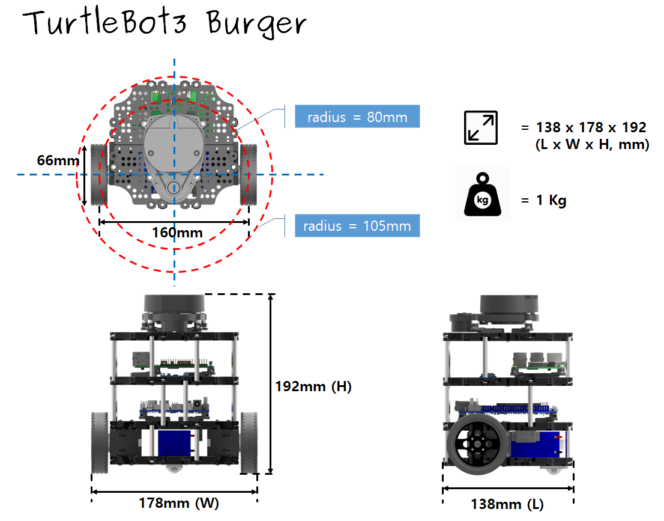
\includegraphics[width=\linewidth]{images/basics/turtlebot3_dimension1.png}
\caption{Turtlebot3 Burger Dimensions \autocite{emanual-turtlebot3-comp}}
\label{fig:turtlebot-dimensions}
\end{figure}
%Source: https://emanual.robotis.com/assets/images/platform/turtlebot3/hardware_setup/turtlebot3_dimension1.png

\begin{figure}[!ht]
\centering
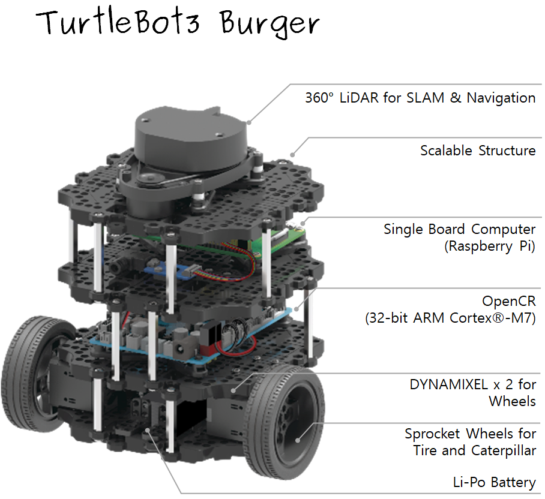
\includegraphics[width=\linewidth]{images/basics/turtlebot3_burger_components.png}
\caption{Turtlebot3 Burger Components \autocite{emanual-turtlebot3-comp}}
\label{fig:turtlebot-components}
\end{figure}
%Source: https://emanual.robotis.com/assets/images/platform/turtlebot3/hardware_setup/turtlebot3_burger_components.png

The complete specifications can be found in the official documentation. The LiDAR sensor is not used for this project.

\subsection{Object Detection}

The following subsections explain the basics of object detection, more specifically the \ac{YOLO} approach.

\subsubsection{YOLO}

While there are many approaches to object detection, the \ac{YOLO} approach stands out. When its paper was released back in 2015 it outperformed many of the existing detectors of that time. The full version is able to detect 45 frames per second and the fast version is detecting 155 frames per second with a Titan X graphics card on the PASCAL VOC dataset while still having more than double the \ac{mAP} than other real-time detectors in that comparison. Compared to its competitors it makes more localisation errors but has less false positives \autocite{yolo}.

\ac{YOLO} only looks once over an image. It consists of one single convolutional neural network that predicts bounding boxes and probabilities. This means that it treats object detection as a regression problem and predicts objects in one single go through in contrast to other detectors which mostly use pipelines with multiple stages \autocite{yolo}.
Unlike many other detectors, \ac{YOLO} does not use a sliding window approach or region proposal-based techniques but sees the complete image. This enables it to make use of contextual information about objects and to not see parts of the image isolated. Therefore it detects less false positives when mistaking background patches for objects. It learns a more generalized representation of objects and can more easily be applied to new domains than other detectors. The downside of this is that it is less accurate on small objects compared to other state-of-the-art systems.

\begin{figure}[!ht]
\centering
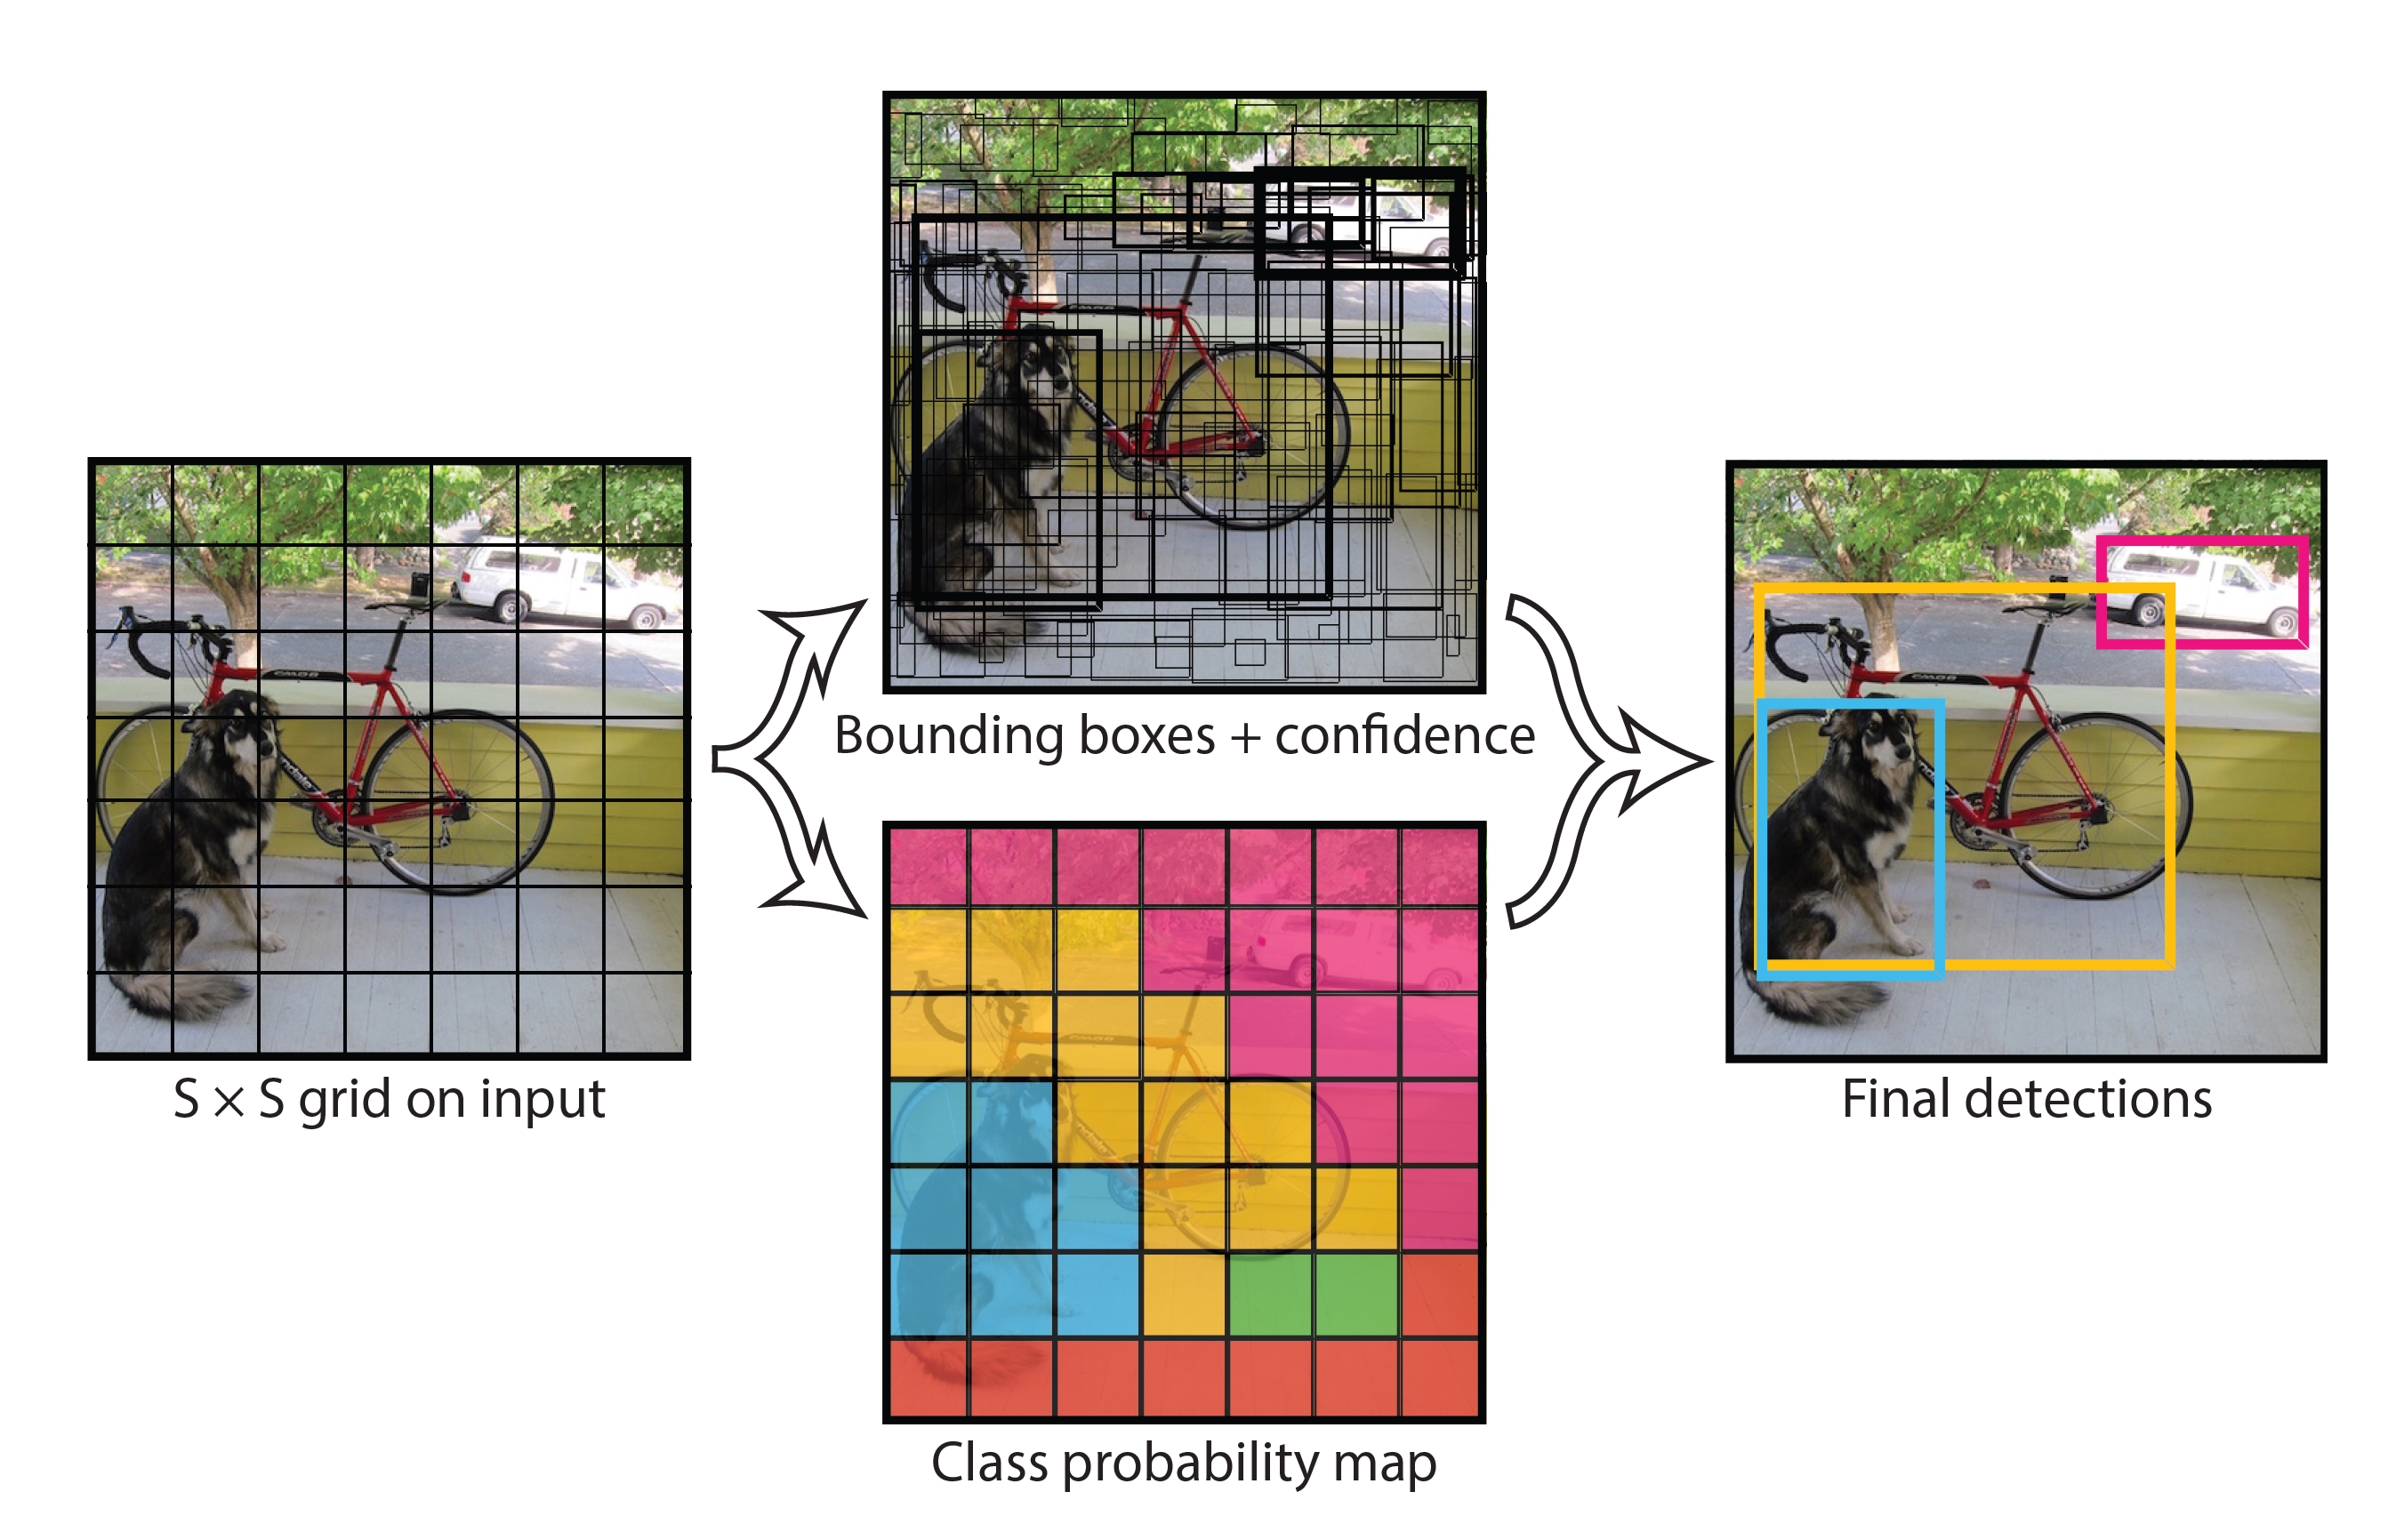
\includegraphics[width=\linewidth]{images/basics/yolo_detection_grid}
\caption{The image is divided into a grid for detecting features. \autocite{yolo}}
\label{fig:yolo_detection_grid}
\end{figure}

In \ac{YOLO} normally separated components for detecting objects are merged into one single neural network. The input image is divided into a \textit{S} x \textit{S} sized grid, where \textit{S} is the size of the grid (\autoref{fig:yolo_detection_grid}) \autocite{yolo}.

Each cell is responsible for detecting the object whose center is located in the corresponding cell. Every cell predicts \textit{B} bounding boxes and their confidence score. These predictions consist of \textit{x}- and \textit{y}-coordinates of the center, width, height and confidence of the bounding box. The confidence represents how confident the system is that the predicted bounding box matches the real object's bounds. Combined with conditional class probabilities a class specific confidence for each bounding box is calculated. These scores represent how likely the class matches the object and how likely the bounds match the bounds of the object (\autoref{fig:yolo_detection_grid}) \autocite{yolo}.

The neural network consists of 26 layers, 24 convolutional layers and two fully connected layers. The initial convolutional layers extract features from the image. To reduce the feature space alternating 1x1 layers are used with 3x3 layers (\autoref{fig:yolo_layers}) \autocite{yolo}.

\begin{figure}[!ht]
\centering
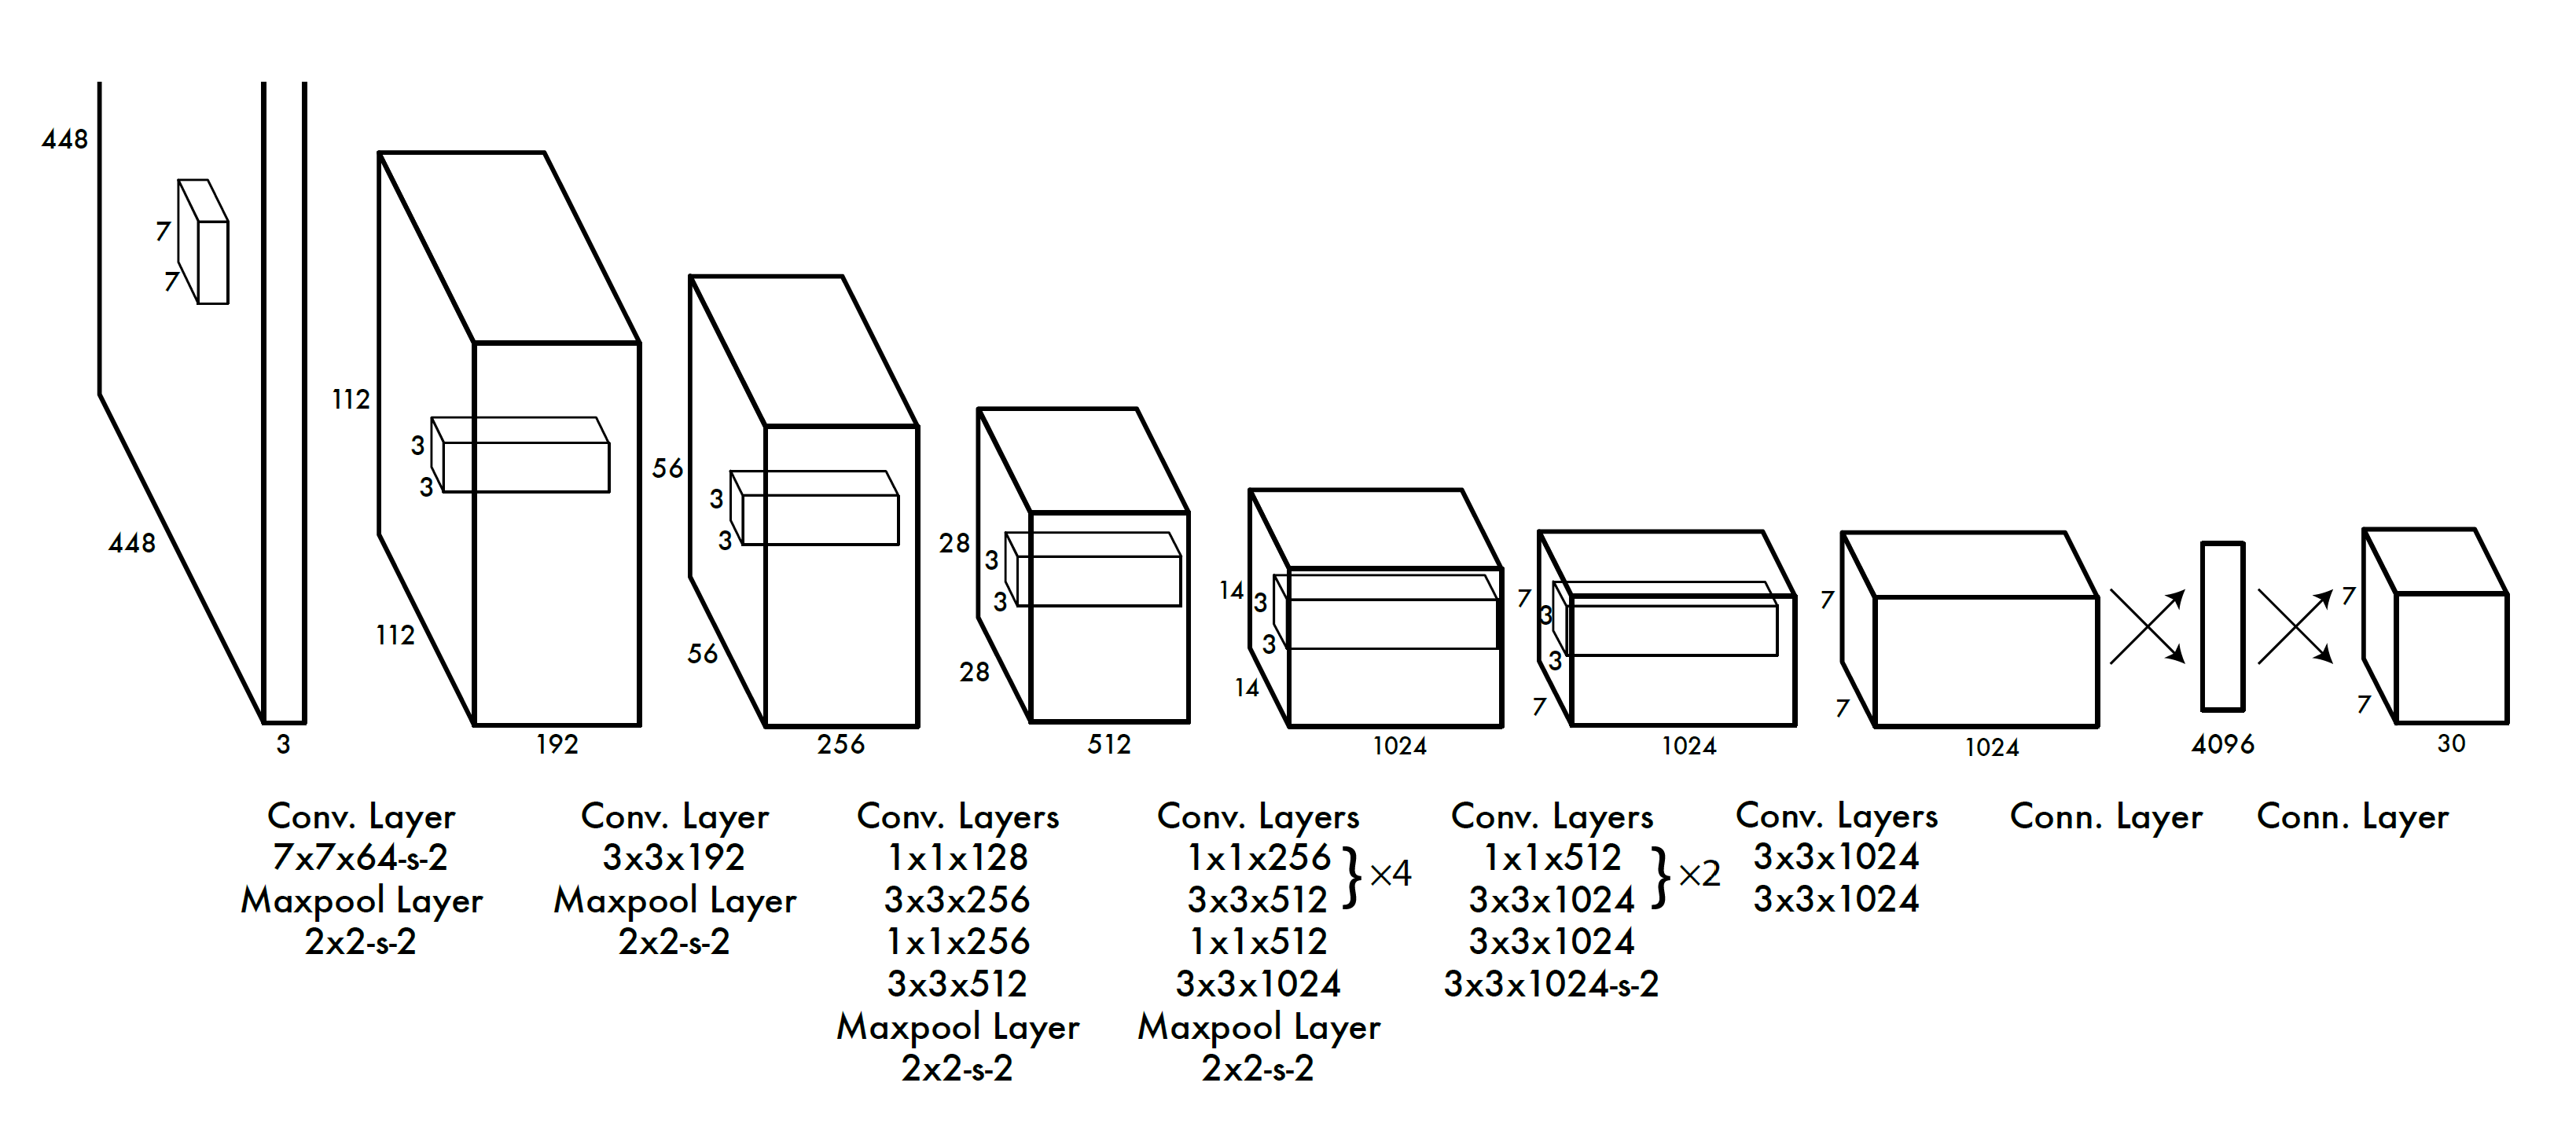
\includegraphics[width=\linewidth]{images/basics/yolo_layers}
\caption{Architecture of the network. \autocite{yolo}}
\label{fig:yolo_layers}
\end{figure}

The fully connected layers predict probabilities and coordinates of the bounding boxes. For the fast version only 9 convolutional layers are used. It is much faster than the full version but also less accurate \autocite{yolo}.

As the training of the network is not of importance in this project it will not be covered in this paper.

The \ac{YOLO} approach also has some limitations. As each cell only predicts two boxes it has problems with multiple objects close to each other, especially when they are small, a flock of birds for example. Objects with unusual aspect ratios are problematic too. Another problem is that the loss function during training treats errors in small and large boxes the same, but a small error in a small box has a much larger impact than a small error in a large box. This leads to incorrect localisations of objects \autocite{yolo}.

\subsubsection{YOLOv4}

As there currently is no paper on the newest version YOLOv5 the rough structure of YOLOv4 will be explained here.

\begin{figure*}[!ht]
\centering
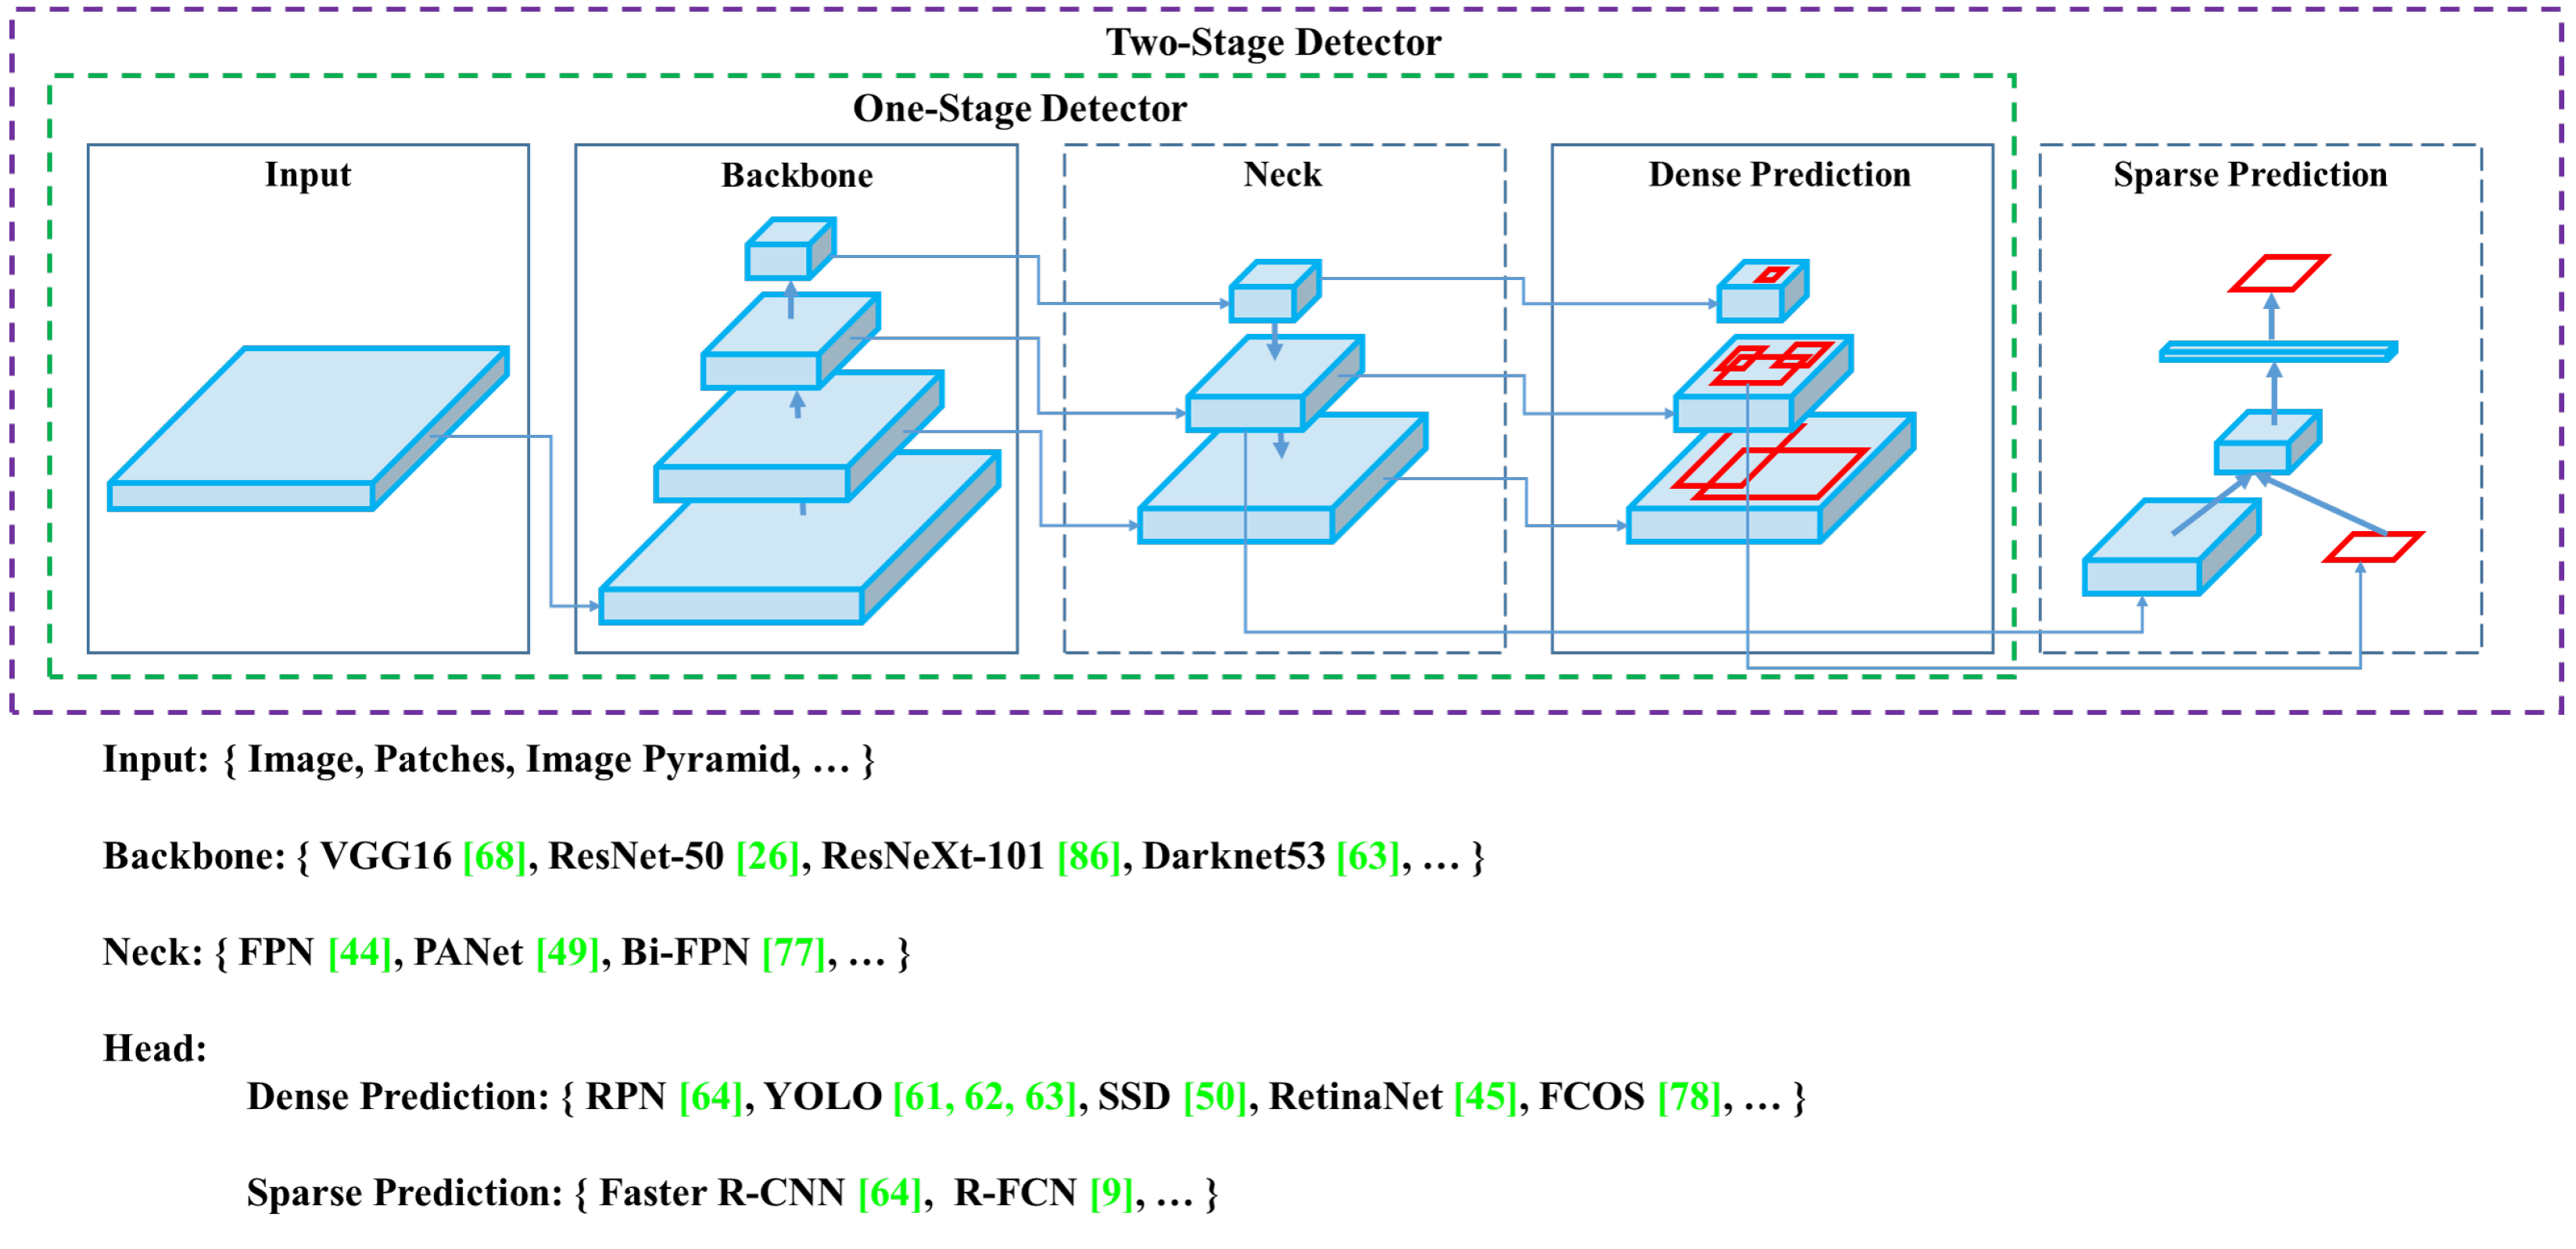
\includegraphics[width=\textwidth]{images/basics/yolov4_architecture}
\caption{Architecture of one- and two-stage object detectors. In the case of YOLOv4 we look at a one-stage detector. The sparse prediction part
therefore is irrelevant in this context. \autocite{yolov4}}
\label{fig:yolov4_architecture}
\end{figure*}

YOLOv4 consists of an input layer, a backbone, a neck and a head (\autoref{fig:yolov4_architecture}). The input layer is a standard input layer. The backbone consists of multiple convolutional layers that are responsible for extracting important features from the input image. The researchers chose the CSPDarknet53 neural network for this task. Following the backbone the neck generates feature pyramids from the extracted features. These pyramids generalize the object scaling. For this stage \ac{SPP} and \ac{PANet} were selected. \ac{SPP} increases the receptive field which describes the area that is looked at at once. A larger receptive field means that not only the object is evaluated but the area around it, therefore a larger context is included. \ac{SPP} separates out the most significant context features. The \ac{PANet} is used for parameter aggregation. Finally the head is used to predict classes and bounding boxes. In YOLOv4 the \ac{YOLO} approach is selected for this task, more precisely YOLOv3 \autocite{yolov4}.

\begin{figure}[!ht]
\centering
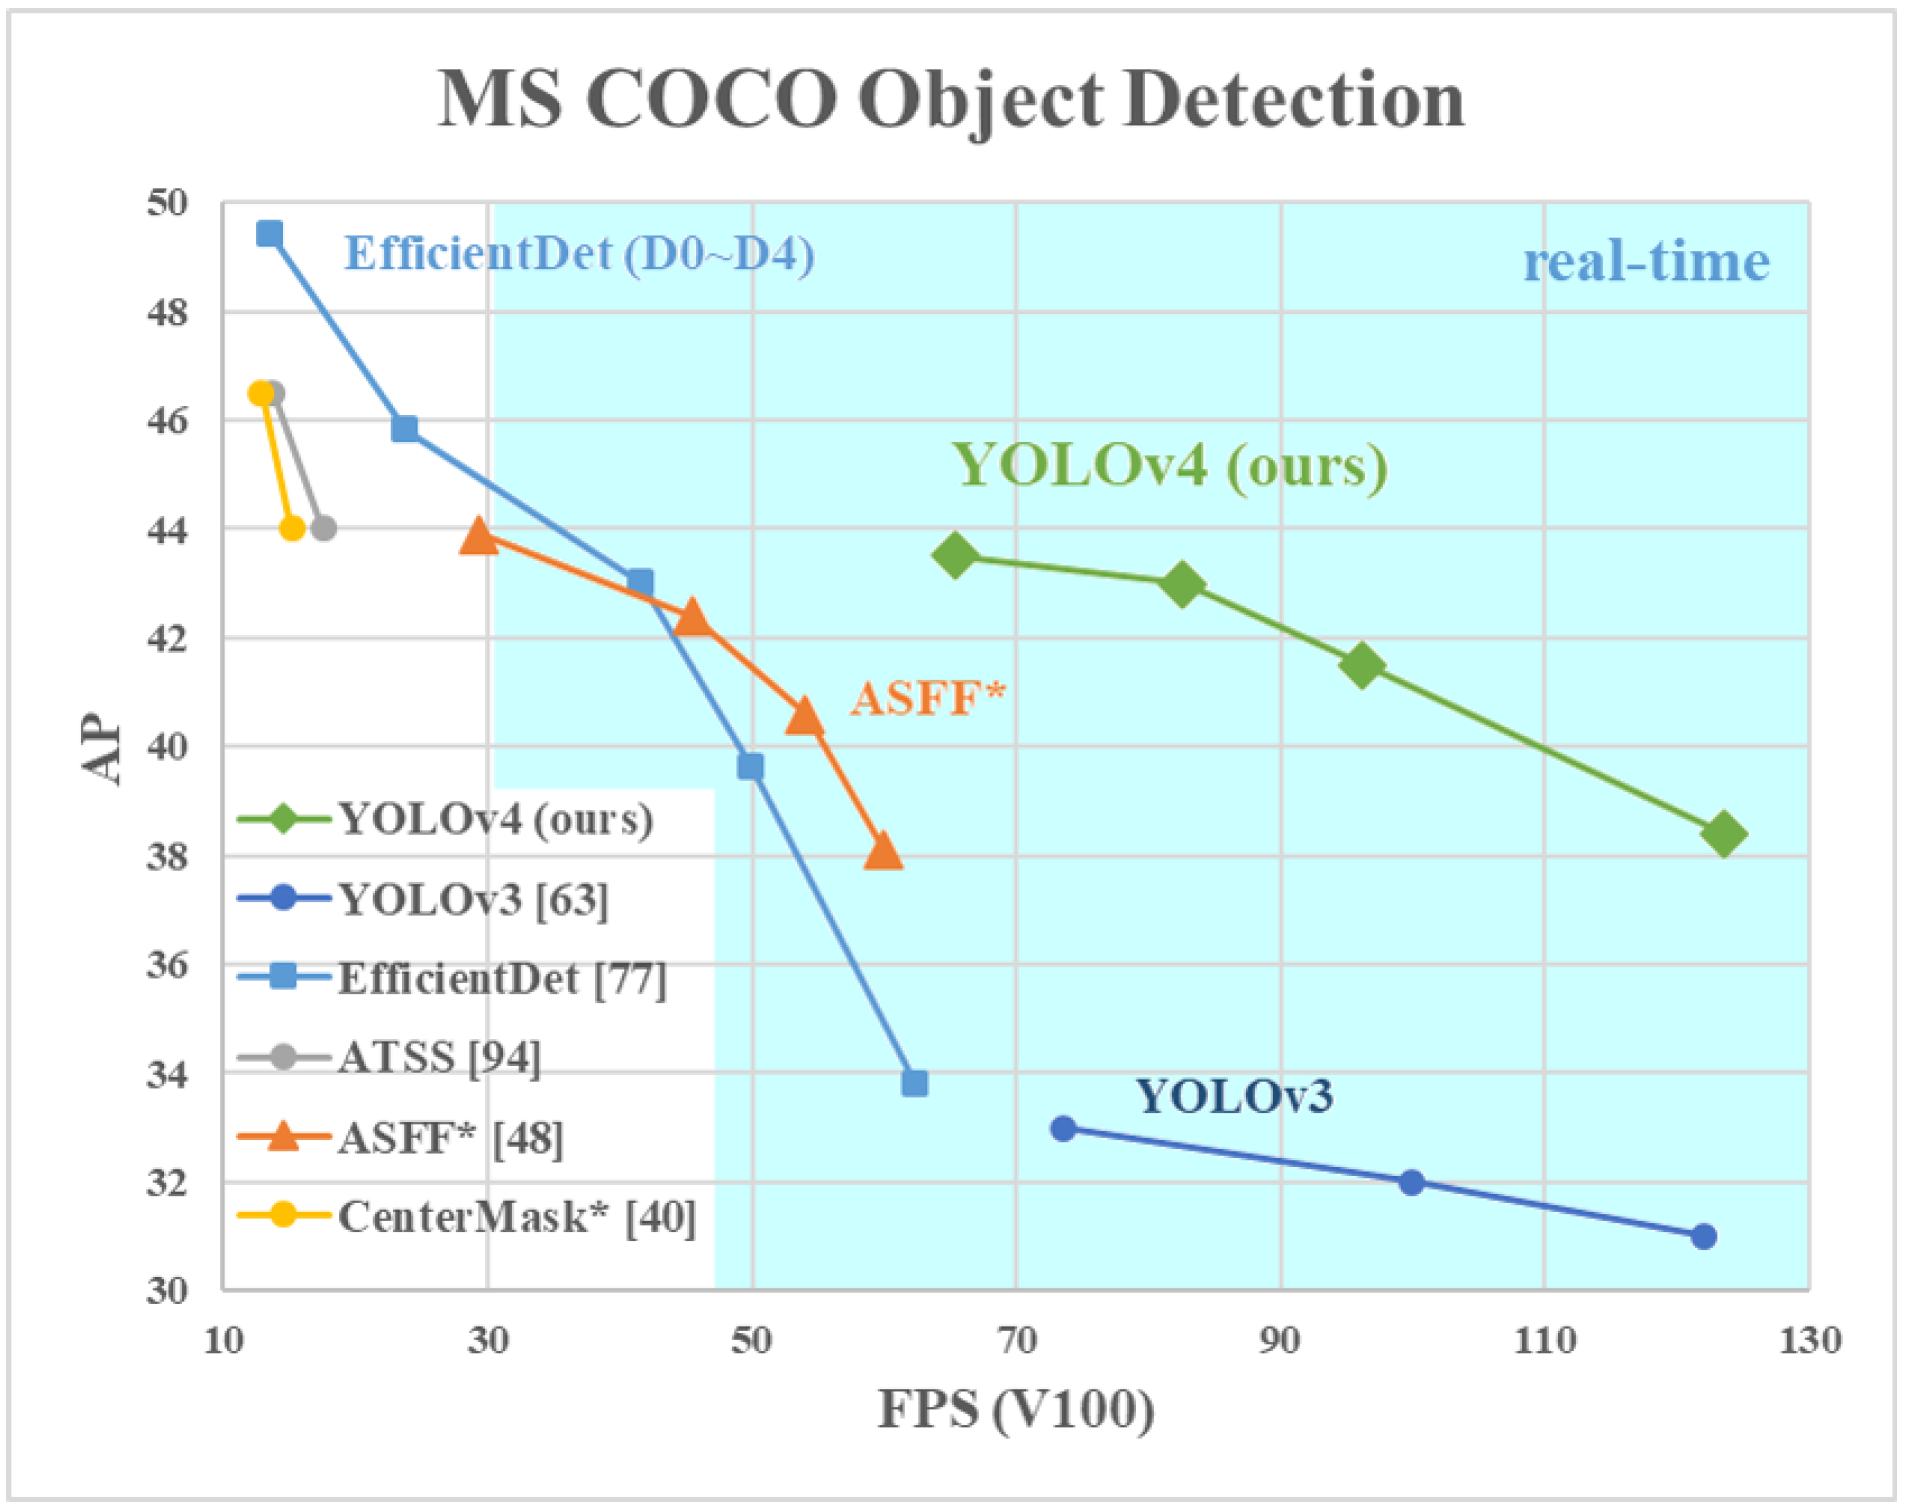
\includegraphics[width=\linewidth]{images/basics/yolo_v4_performance}
\caption{Performance comparison between YOLOv4, the predecessor YOLOv3 and other state-of-the-art detectors on the MS COCO dataset. \autocite{yolov4}}
\label{fig:yolo_v4_performance}
\end{figure}

As seen in \autoref{fig:yolo_v4_performance} YOLOv4 outperforms all other state-of-the-art detectors. Although EfficientDet, CenterMask and ATSS are able to perform better regarding the average precision they lack the speed of YOLOv4. YOLOv3 offers a comparable speed but at a much lower average precision. A more detailed comparison can be found at the researchers GitHub repository (https://github.com/AlexeyAB/darknet) \autocite{yolov4}.

\subsubsection{YOLOv5}

Although there currently is no paper on YOLOv5 the editorial team of TOWARDS AI published an article about its architecture.

YOLOv5 is a single-stage object detector too, so the rough overview of \autoref{fig:yolov4_architecture} can be applied. 
It consists of a backbone for feature extraction, a neck for feature pyramids that help with object scaling and unseen data and a head for predicting bounding boxes, classes and confidence. For the backbone the \ac{CSPNet} was selected, for the neck \ac{PANet} and for the head YOLOv3 again. In the hidden layers the Leaky ReLU function was selected as activation function, in the final detection layer a sigmoid function is used \autocite{towards_ai}.

\begin{figure}[!ht]
\centering
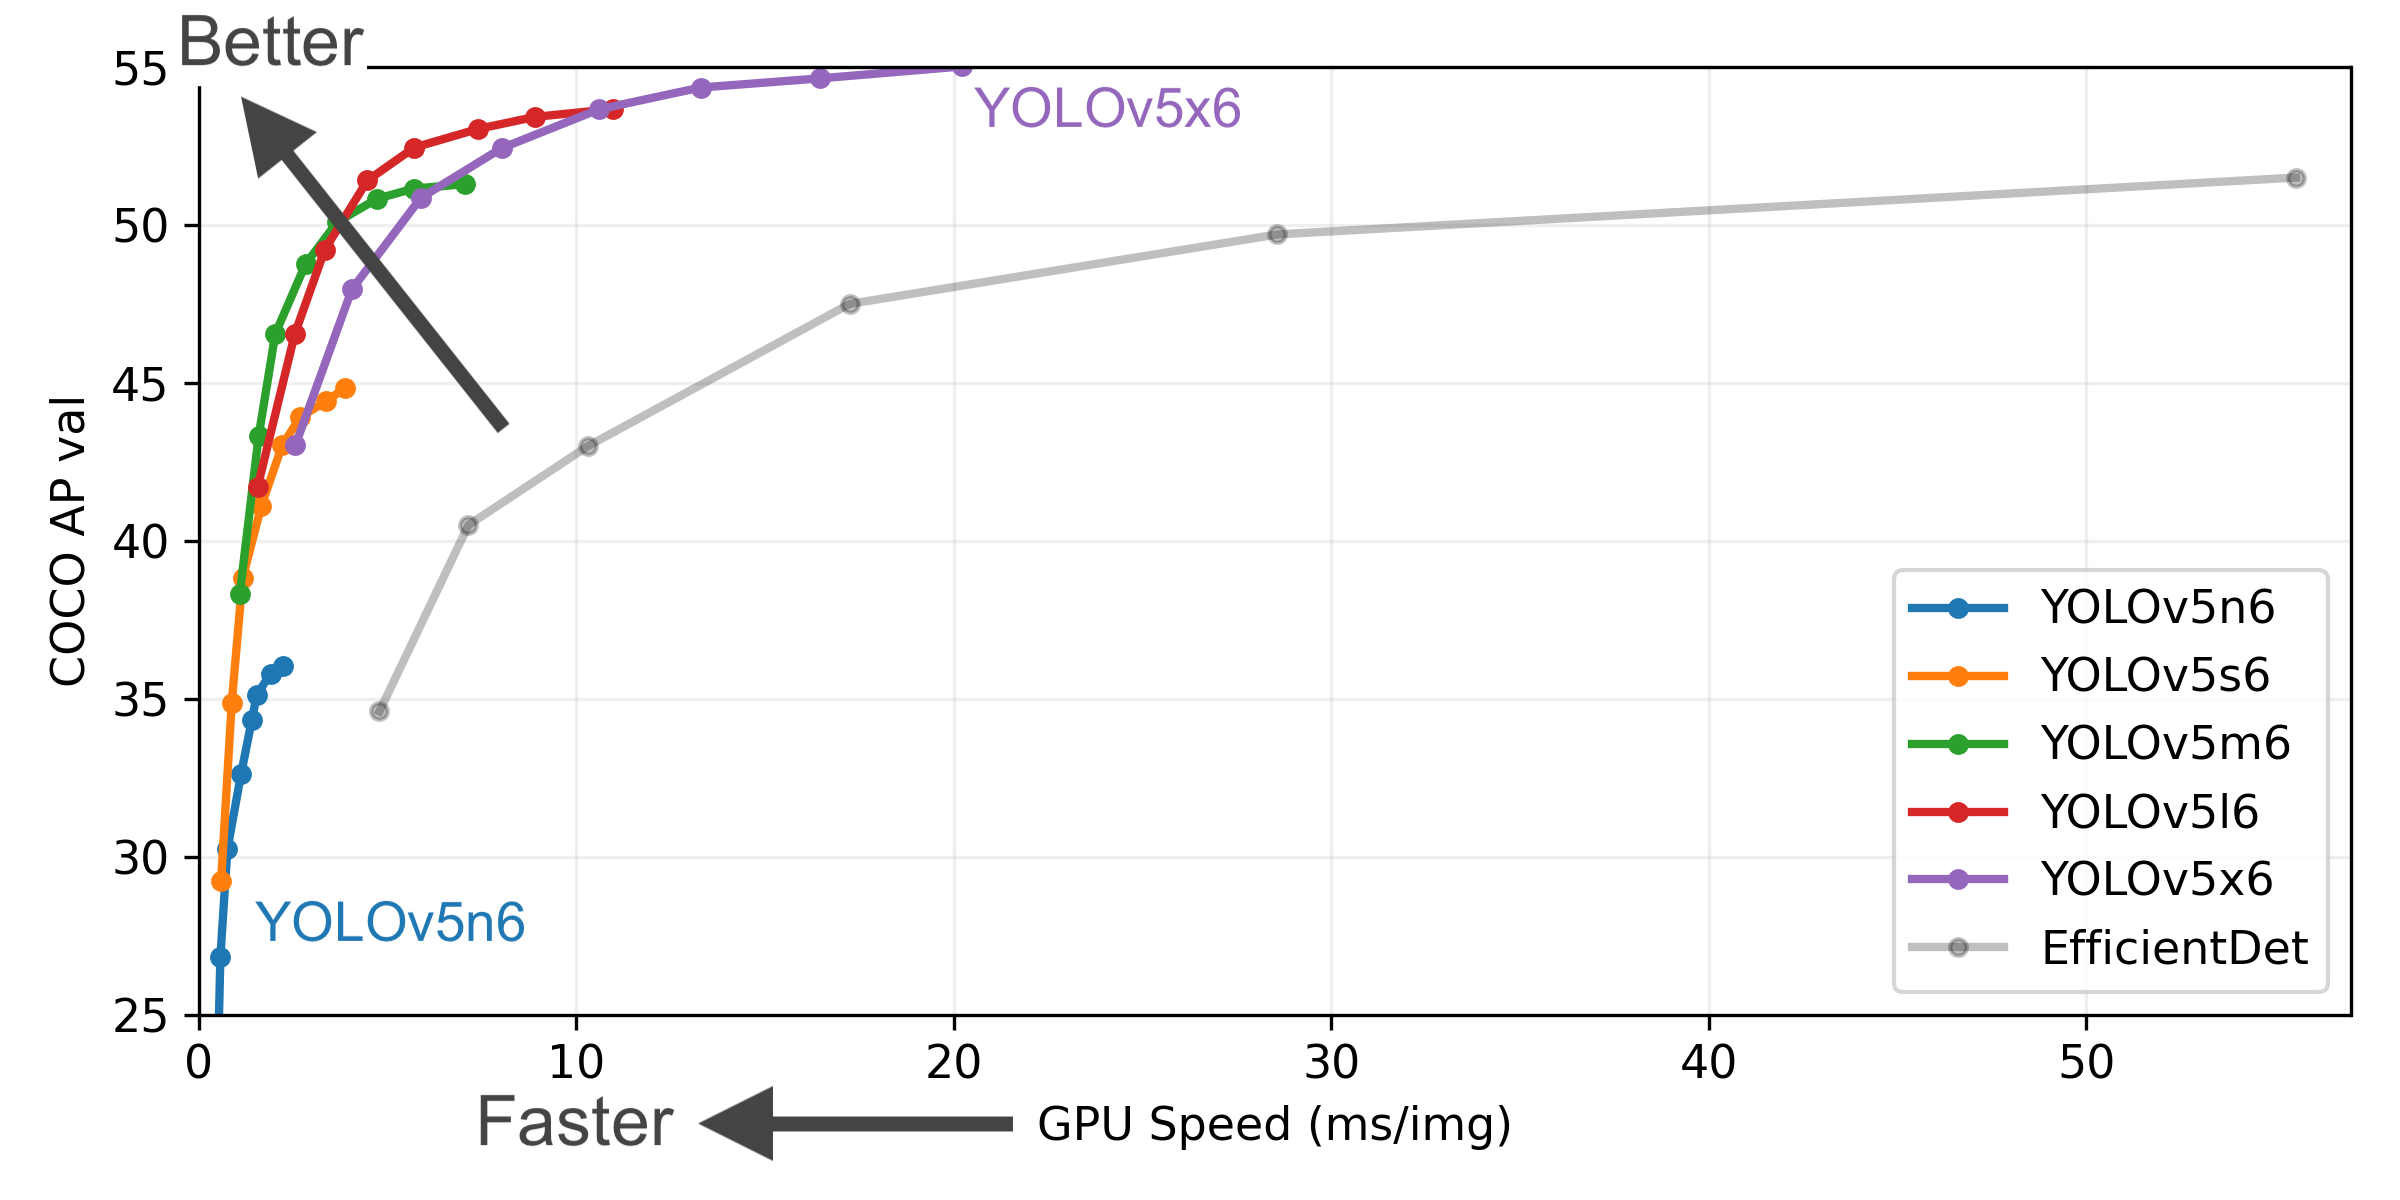
\includegraphics[width=\linewidth]{images/basics/yolov5_comparison}
\caption{Comparison between different YOLOv5 models and EfficientDet. It is important to notice that the x-axis is measured in milliseconds per image, not images per second as in \autoref{fig:yolo_v4_performance}. \autocite{ultralytics}}
\label{fig:yolov5_comparison}
\end{figure}

There are multiple pretrained models of YOLOv5 (YOLOv5n6, YOLOv5s6, YOLOv5m6, YOLOv5l6 and YOLOv5x6). The researchers of YOLOv5 show a performance comparison between the different YOLOv5 models and EfficientDet \autoref{fig:yolov5_comparison}). All YOLOv5 models perform faster than EfficientDet with some also having a better average precision \autocite{ultralytics}.


\section{Turtlebot Setup for the Project}

The following chapter provides technical details about the hard- and software used to run the robot and control its motion.

\subsection{Turtlebot Configuration}

The Raspberry Pi requires relatively little setup. The official documentation provides a link to the Raspberry Pi \ac{OS} (Raspbian OS). The image includes \ac{ROS} Neotic and can be burned to the SD card via the Raspberry Pi Imager. After a successful boot, the network settings need to be configured to connect to a nearest WiFi. The exact network setup is described in the Network Setup chapter below. After that, it is possible to connect to the Raspberry Pi via \ac{SSH}, which makes further changes to the configuration easier.
The only configuration ROS needs is the IP addresses for both the ROS master and Raspberry Pi itself as well as the Turtlebot model name.

{\scriptsize
\begin{lstlisting}[language=sh,frame=single,caption=Environment Variables,label=code:env]
export ROS_MASTER_URI=http://{IP_ADDRESS_OF_REMOTE_PC}:11311
export ROS_HOSTNAME={IP_ADDRESS_OF_RASPBERRY_PI_3}
export TURTLEBOT3_MODEL=${TB3_MODEL}
\end{lstlisting}}

After that, \lstinline|roslaunch turtlebot3\_bringup turtlebot3\_robot.launch| starts \ac{ROS}, which tries to establish a connection to the remote PC (ROS master). Basic moving operations can be tested with \lstinline|turtlebot3\_teleop\_key| which might run into an error as the default user \enqoute{\textit{ubuntu}} on the Turtlebot image does not have the proper \ac{tty} permissions. The problem can be solved by adding \enqoute{\textit{ubuntu}} to the \enqoute{\textit{root}} user group. This can be done by executing the following command: \lstinline|sudo usermod -aG root ubuntu|. The normal group used for this is called \enqoute{\textit{dialout}} and is not set for \ac{tty}.

The robot is equipped with a Raspberry Pi Cam mounted to the front of the vehicle with a slider to adjust the position of the camera up and down. The slider is necessary to find the optimal position for object detection. A fork with masking tape is mounted to the front of the robot to pick up and hold a tennis ball. The below picture shows the additional modifications to the robot.

\begin{figure}[!ht]
\centering
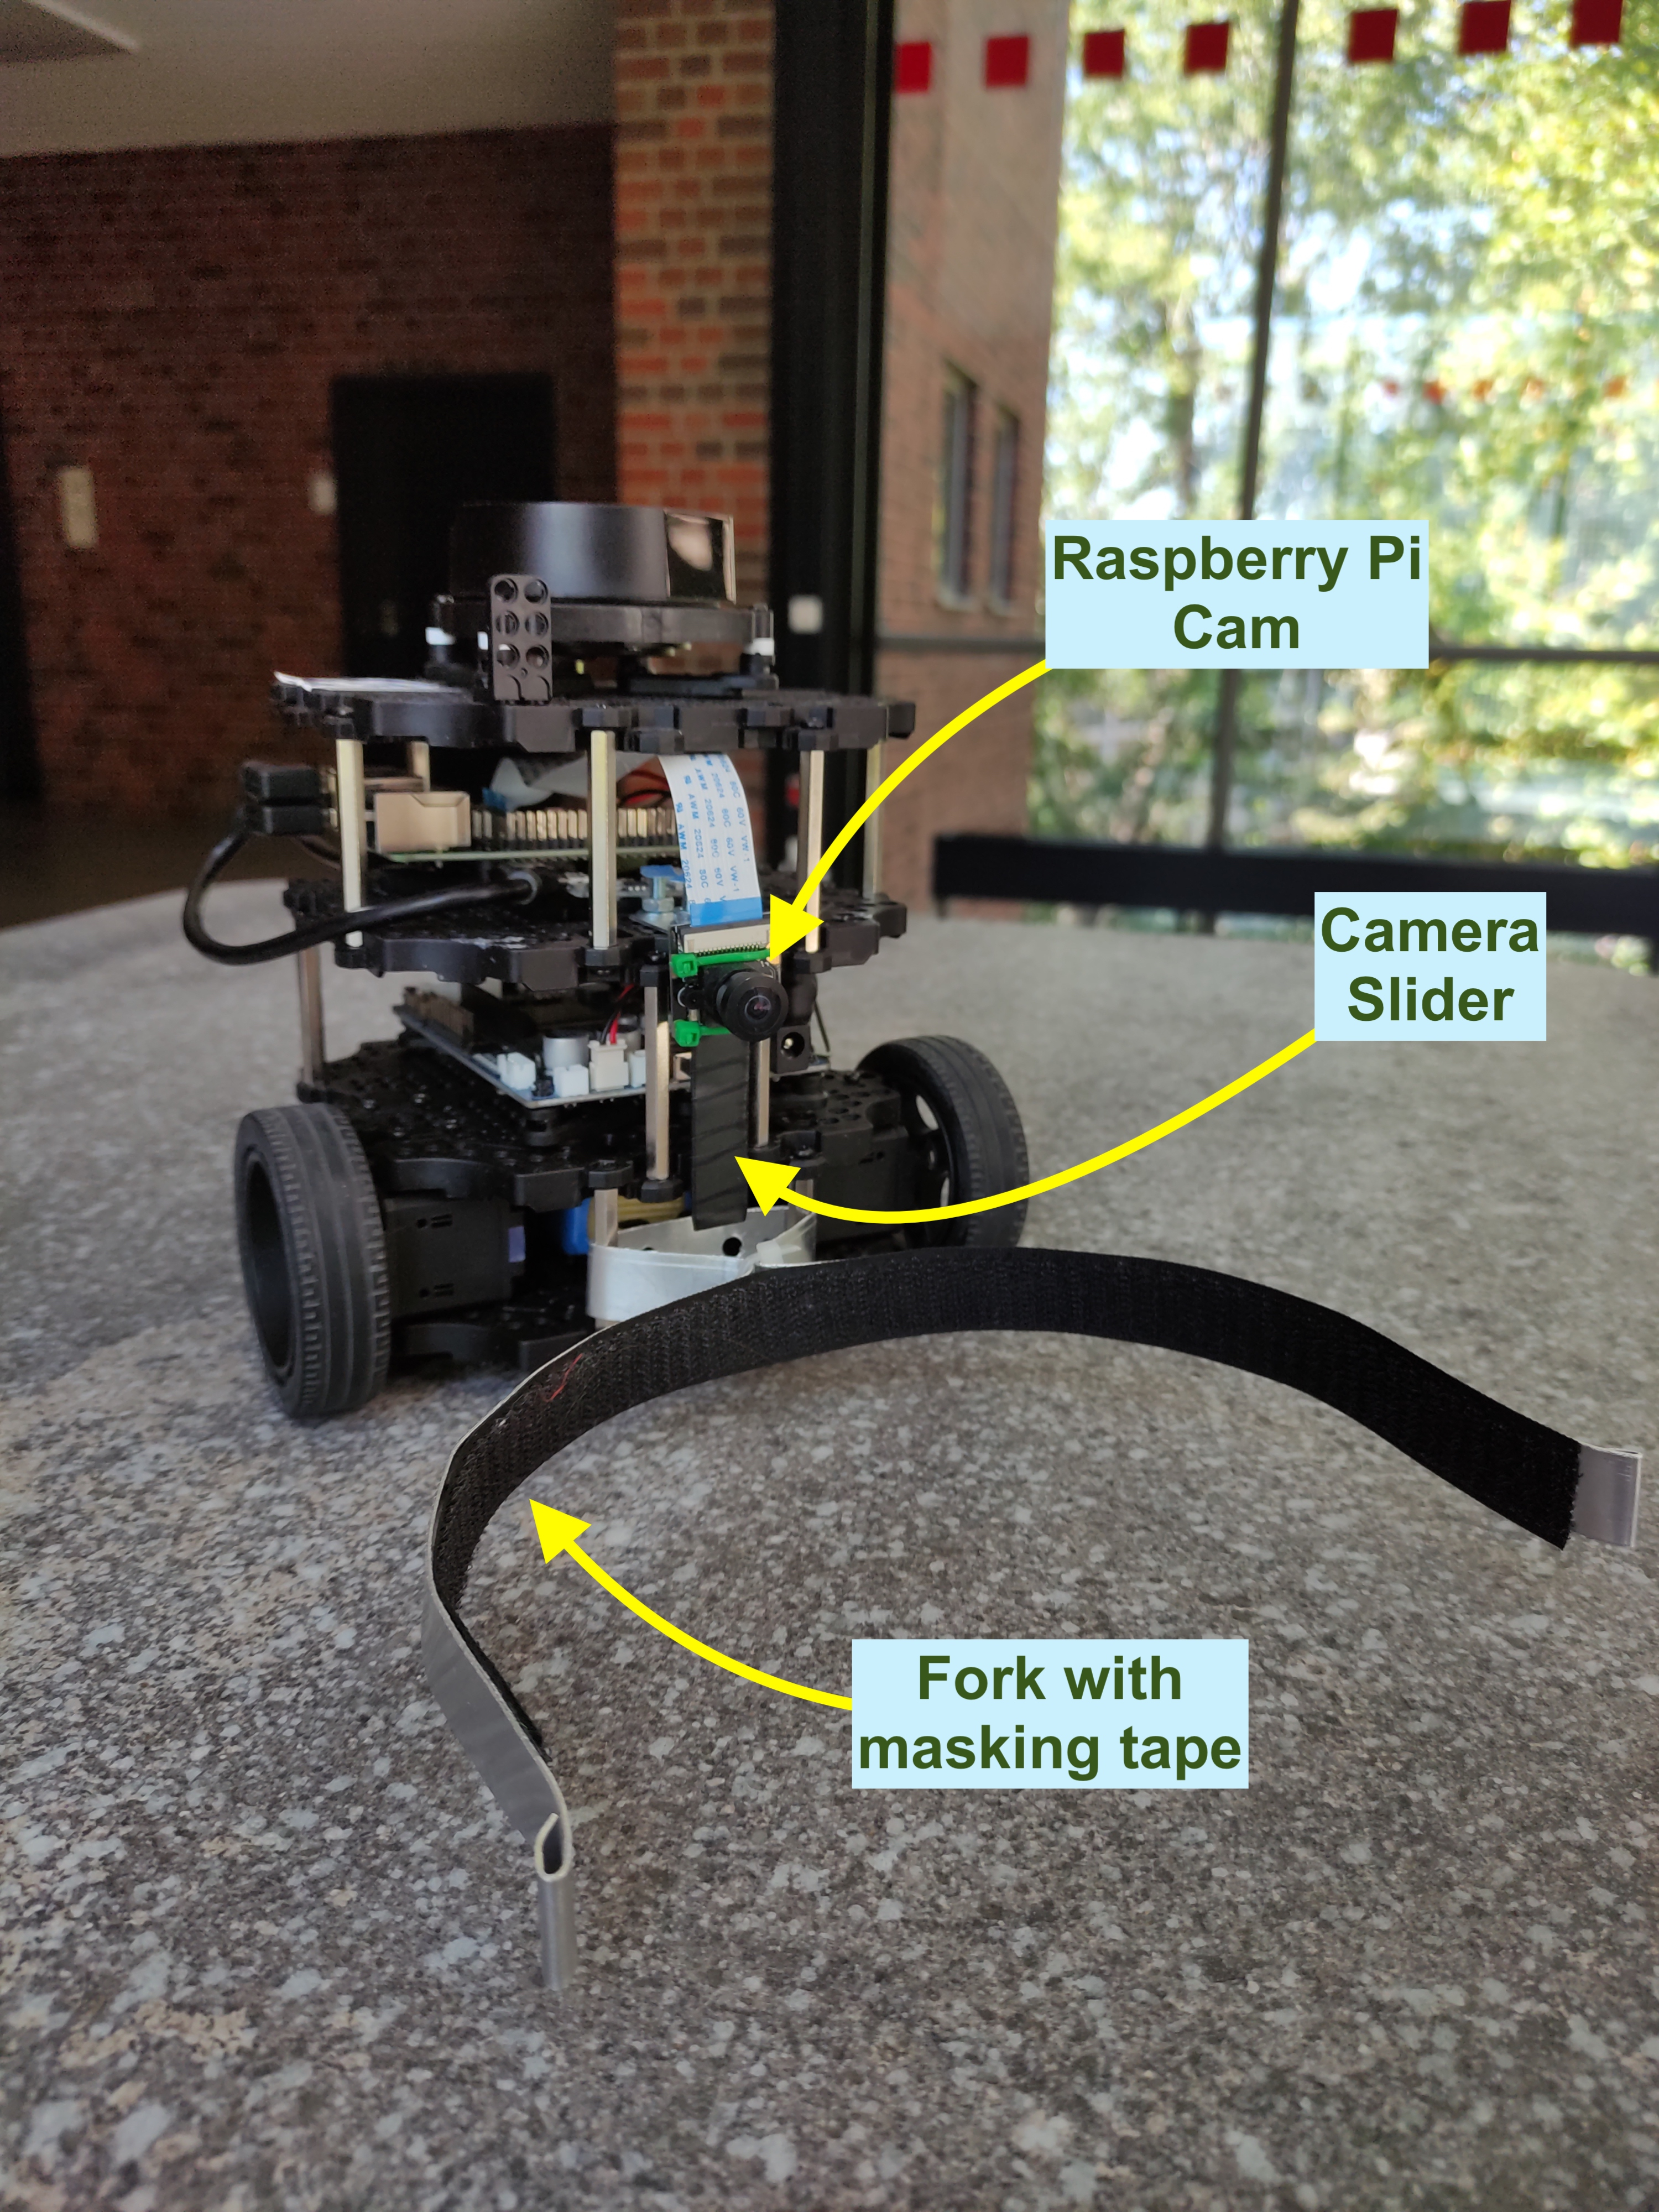
\includegraphics[width=\linewidth]{images/turtlebot-setup/ball-schubser_front_side_new_desc.jpg}
\caption{Turtlebot Additional Components}
\label{fig:turtlebot-add-components}
\end{figure}

\subsection{Network Setup}

The Raspberry Pi has WiFi capability and is connected to a small home router or alternatively to a mobile phone hotspot. The Docker containers running on the remote PC rely on its host network and thus operate in the same subnet.

\begin{figure}[!htb]
\centering
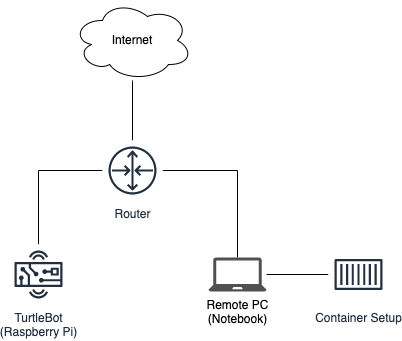
\includegraphics[width=\linewidth]{images/turtlebot-setup/network_setup.png}
\caption{Network Map used for the Robot Setup}
\label{fig:network-setup}
\end{figure}

\subsection{Containerized Application Setup with Docker}
\label{sec:container-setup}
Docker allows for a simplified setup and development of the robot. Therefore docker runs on the development computer, and the turtlebot connects to the created ROS Nodes.

\begin{figure}[!ht]
\centering
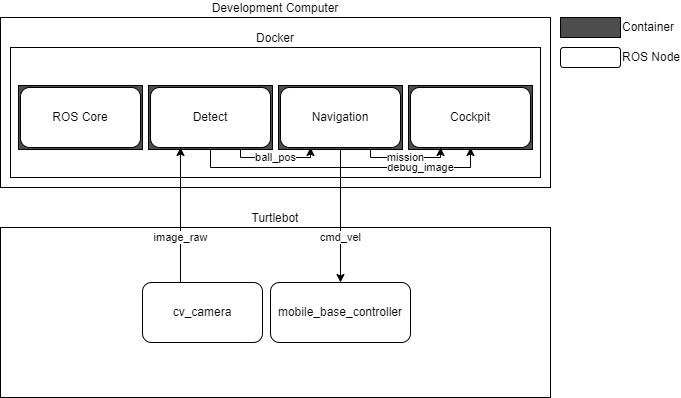
\includegraphics[width=\linewidth]{images/turtlebot-setup/docker-setup.png}
\caption{Development Computer and Turtlebot Setup}
\label{fig:dev-pc-turtlebot}
\end{figure}
%link: https://1drv.ms/u/s!Ar0XPmCdJWduifRsBllZFgas6HMQ1w?e=fnWUfO

In the previous image, we can see the docker setup connecting the development computer with the Turtlebot. Docker runs not only the ROS core but also three other nodes.

First, the detection node publishes values of the detected object. The navigation node then uses this data to update the robot's rotation and speed accordingly. Lastly, there is the Cockpit node, which uses the data of the detect and navigation nodes to create a helpful view for debugging and presenting the final robot.

In addition to the ROS nodes created in docker, multiple ROS nodes are running on the Turtlebot. First, the camera node publishes the camera images. Second, the steering endpoint uses the data published by the navigation node to control the robot's behavior.
The ROS nodes on the Turtlebot and the ROS nodes on the development computer are communicating through  \acf{TCP}\cite{ros-technical-overview}. This is possible because the docker containers are using the host network, which is enabled through the compose property `network\_mode: host` that is set for all containers\cite{docker-host}.

All of the docker containers are created with the help of the docker-compose file that can be found in the Appendix as \autoref{code:compose}.

In addition to an easy setup, docker-compose allows for an easy transfer of all needed ROS nodes from one computer to another.

%====

\subsection{Startup Automation and Development}
Starting up the Turtlebot with all the required nodes to run the robot is not a simple task. Therefore different steps like using docker and creating automation scripts are taken. The first step is to use Docker to set up the ROS Core, the detection, the navigation, and the cockpit nodes. Because of docker, all these nodes could be started by running `docker-compose up -d`. The containers and the communication between them are explained in \autoref{sec:container-setup} and especially in \autoref{fig:dev-pc-turtlebot}.
The second step is to turn on the turtlebot. This is the only step that could not be simplified because it is something that has to be done in the real world.
The last step is to run the different nodes that are needed on the Turtlebot. These are first the Turtlebot core and then the camera. For this, the following config.sh, cam.sh and launch.sh scripts are created, and both cam.sh and launch.sh could be simply run to start all necessary systems on the turtlebot. The config.sh set environment variables and is automatically run as part of both scripts.

{\scriptsize
\begin{lstlisting}[language=sh,frame=single,caption=config.sh,label=code:config]
#! /bin/bash
export ROS_MASTER_URI=http://192.168.31.34:11311

export ROS_IP=192.168.31.4

export LDS_MODEL=LDS-01
export TURTLEBOT3_MODEL=burger
\end{lstlisting}
}

{\scriptsize
\begin{lstlisting}[language=sh,frame=single,caption=cam.sh,label=code:cam]
#! /bin/bash
source ./config.sh

rosparam set cv_camera/device_id 0
rosrun cv_camera cv_camera_node
\end{lstlisting}
}

{\scriptsize
\begin{lstlisting}[language=sh,frame=single,caption=launch.sh,label=code:launch]
#! /bin/bash
source ./config.sh

roslaunch turtlebot3_bringup turtlebot3_core.launch
\end{lstlisting}
}

For a simplified development, the watchdog was used to rerun the containers start command as soon as the used file was changed. For this, the entry point to a node had to be defined as follows (inside the docker-compose.yml): \lstinline|command: /watchdog.sh cockpit.py|. Watch dog is a python package for monitoring and reacting on file changes.\cite{watchdog}

%===

\subsection{Robot Navigation}
As visible in \autoref{fig:dev-pc-turtlebot} the navigation node is based on the target positon information retirieved inside the detection node. The target position represents the position inside the image in percentage. For that 0,0 is the lower left corner of the image and 100, 100 to upper right corner. If the target would be exactly in the middle of the image it would be represented as 50,50.
For the navigation node both \textit{x} and \textit{y} percentage are important to decide how to navigate. If a target is visible on the right side of the image, meaning over 50, the robot will turn right, if it is below 50 it will turn left. In case there is no target visible at all, the robot will start turning in the direction the target was last seen, until the target is visible again.
This decsion tree is also represented in the following image:

\begin{figure}[!ht]
\centering
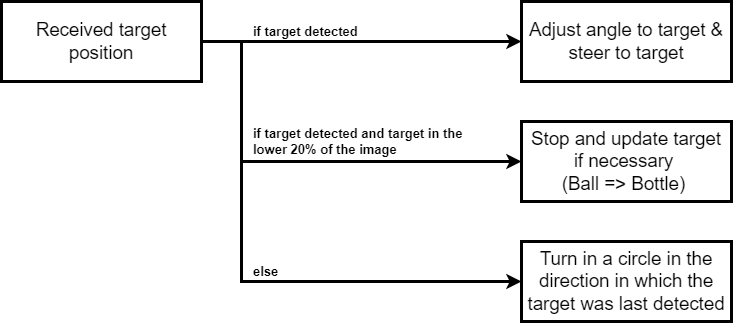
\includegraphics[width=\linewidth]{images/turtlebot-setup/navigation-tree.png}
\caption{Navigation Tree}
\label{fig:navigation-tree}
\end{figure}
%link: https://1drv.ms/u/s!Ar0XPmCdJWduifUkDkNhmOXm4zfyDA?e=tA43yK

%===

The below image shows the nodes and topics as they are defined in ROS. The arrows moving from left to right show the information flow from the camera node, which receives the raw image and publishes it to the detect node, where it is processed and the ball position is published to the control node. The detect node also sends the image to the mission cockpit. The control node then publishes the direction and velocity to the Turtlebot core and the mission statement to the cockpit.

\begin{figure}[!ht]
\centering
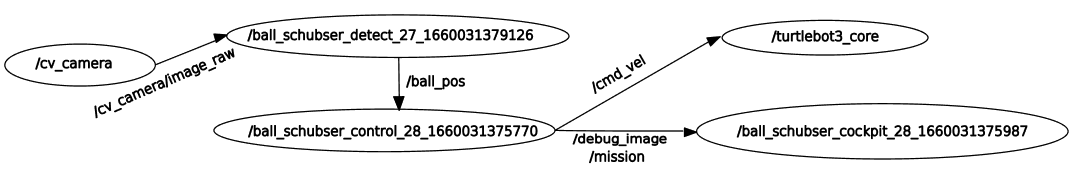
\includegraphics[width=\linewidth]{images/turtlebot-setup/ros_graph.png}
\caption{ROS Nodes and Topics Graph}
\label{fig:ros-rqt-graph}
\end{figure}

\subsection{Cockpit}
The cockpit was introduced for debugging reasons and for a better explanation of what is happening. The cockpit shows information about the robot's current state, the camera picture, and the different objects recognized by the detection node.

\begin{figure}[!ht]
\centering
\includegraphics[width=\linewidth]{images/turtlebot-setup/cockpit.png}
\caption{Cockpit showing bounding boxes of ball, bottle and mug}
\label{fig:cockpit}
\end{figure}

The Cockpit is viewable inside the web browser and is based on Flask, a Python framework for creating web servers. Flask has different functionalities, like automatically updating the shown image when a new one is available. It enables a \enqoute{live stream} of images by always showing the latest image retrieved by the detection node through the debug\_image topic. The detection node modifies the image with bounding boxes in different colors. Each color represents a different class:

\begin{itemize}
    \item red: bottle
    \item green: ball
    \item blue: mug
\end{itemize}

The image containing the bounding boxes is then modified with a mission text published by the navigation node on the mission topic. All of the modifications on the image are done with OpenCV.

\subsection{Different Setup Approaches and Problems}

Installing large and complex software packages like \ac{ROS} and \ac{YOLO} directly onto a computer occupies a lot of space. It makes it difficult to switch between versions and to make changes to the general infrastructure setup. To solve this issue a containerized setup is implemented, besides changing the configuration, in addition this makes it easier to move the entire setup between computers.
Slow transfer rates between the remote computer and the Turtlebot do often cause malfunctions in the navigation, as the robot is receiving delayed updates from the remote computer. Moving the setup onto the Raspberry Pi didn’t bring any improvements as the computing power becomes a new bottleneck as the image processing with YOLO takes up to 6s, compared to a few milliseconds on the remote computer. So through a process of elimination, it was established that the best solution was offloading the processing job with the biggest bottleneck being the network connection. As it is not clear what exactly causes the delays on the network, no further investigations were pursued. This problem might be overcome in the future by a newer or different single-board computer e. g. the NVIDIA Jetson or a different setup with a better router, WiFi chips, and computing power. In the meantime working with a remote computer is indispensable.
\section{Detection handling}

This section describes the approach of the object detection. The first subsection is about the selection of a \ac{YOLO} version for this project. Then the detection and processing of the target objects is described.

\subsection{Selecting a YOLO version}

At first YOLOv4 was selected because it is well documented and very popular with the machine learning community. But soon  performance problems occured when trying to detect objects on multiple images per second. While the tiny model for YOLOv4 is much faster than the full model it is also less accurate. Because there were already problems with detecting small objects further away, the tiny YOLOv4 was off the table.

The solution came in the form of YOLOv5. Although it is not as well documented as YOLOv4 the setup was easy and quick. YOLOv5s6 was selected due to the balanced tradeoff between speed and average performance as seen in \autoref{fig:yolov5_comparison}. 

Before implementing it tests to compare YOLOv5 to YOLOv4 were executed on a GTX 1080 using three images from a testing setup. They show a tennis ball in a room full of other objects and look similar to \autoref{fig:detection_bounding_box_rendered}. For testing the performance both models detect all objects in three images 1000 times. The time for each prediction and the confidence of the detected ball was summed up separately and averaged out at the end. The results for the first test run are as following:

\textit{YOLOv4}: average time per prediction:   \textit{98.51ms}, average confidence: \textit{0.79228}

\textit{YOLOv5}: average time per prediction: \textit{172.12ms}, average confidence: \textit{0.84767}

These results were unexpected and soon the reason for this anomaly was discovered: The YOLOv4 implementation in use is implemented in tensorflow which utilizes the GPU for processing, while YOLOv5 is implemented in pytorch, which in the setup of this project only uses the CPU. As the goal was running the detection directly on the Raspberry Pi, the results of a benchmark with GPU support were not useful. After disabling the GPU both models ran on an Intel Core i7-6700K with 4.00GHz. The results were much more as expected:

\textit{YOLOv4}: average time per prediction: \textit{418.00ms}, average confidence: \textit{0.79228}

\textit{YOLOv5}: average time per prediction: \textit{173.94ms}, average confidence: \textit{0.84767}

These results showed that YOLOv5 clearly is the better choice due to being much faster and having slightly better precision.


\subsection{Detecting and processing target objects}

The detection runs on a separate \ac{ROS} node. The node receives an image from the pycam node as an image message. Before being able to process the image any further it has to be converted into an opencv image and flipped horizontally because the py cam is mounted upside down.

There are four object classes that are relevant to the system that can be detected with YOLOv5 trained on the MS COCO dataset. Following is a list with the corresponding index numbers of the classes:


\begin{itemize}
  \item sports ball = 32
  \item bottle = 39
  \item wine glass = 40
  \item cup = 41
\end{itemize}

The results are returned as a pandas dataframe. An example for printed results of a prediction can be seen in \autoref{table:detection_df} and their corresponding bounding boxes in \autoref{fig:detection_bounding_box_rendered}.

\begin{table*}[h]
  \caption{Results of prediction of \autoref{fig:detection_bounding_box_rendered}.}
  \label{table:detection_df}
  \renewcommand{\arraystretch}{1.2}
  \centering
  \sffamily
  \begin{footnotesize}
    \begin{tabularx}{0.7\textwidth}{l L L L L L L L}
      \toprule
      \textbf{id} & \textbf{xmin} & \textbf{ymin} & \textbf{xmax} & \textbf{ymax} & \textbf{confidence} & \textbf{class} & \textbf{name}\\
      \midrule
      0 & 243.6600 & 233.1874 & 263.4035 & 253.4699 & 0.8300 & 32 & sports ball \\
      1 & 71.7961 & 0.0000 & 178.5337 & 253.5528 & 0.7211 & 0 & person \\
      2 & 228.8112 & 55.9412 & 250.8915 & 75.6965 & 0.4448 & 74 & clock \\
      3 & 6.2497 & 103.5277 & 73.3023 & 142.8823 & 0.3524 & 56 & chair \\
      \bottomrule
    \end{tabularx}
  \end{footnotesize}
  \rmfamily
\end{table*}

\begin{figure}[!ht]
\centering
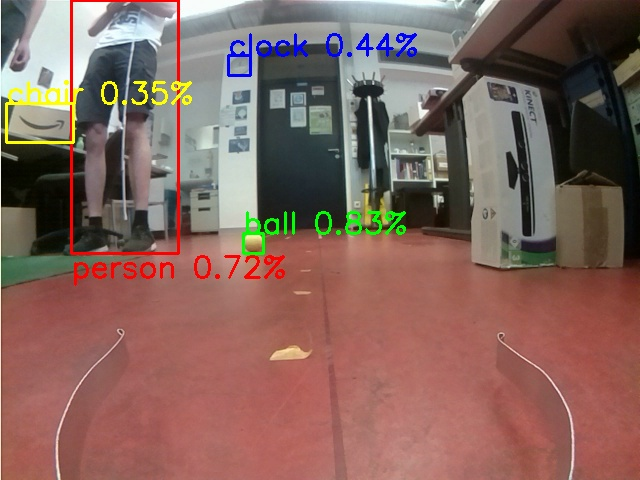
\includegraphics[width=\linewidth]{images/implementation/detection_bounding_box_rendered}
\caption{Rendered bounding boxes of detections.}
\label{fig:detection_bounding_box_rendered}
\end{figure}


If multiple sports balls are detected the detections are ordered by the \textit{y}-axis position of the lower bounding box border of the detection. Then the detection with the lowest position is selected. Lowest meaning highest \textit{y}-value, as the \textit{y}-axis starts at the top edge of the image. The sports ball with the lowest position should be the one closest to the camera due to the perspective of the view from the camera. This assumption should be correct for most cases on a flat plane as it is the case in our testing environment.


\begin{figure}[!ht]
\centering
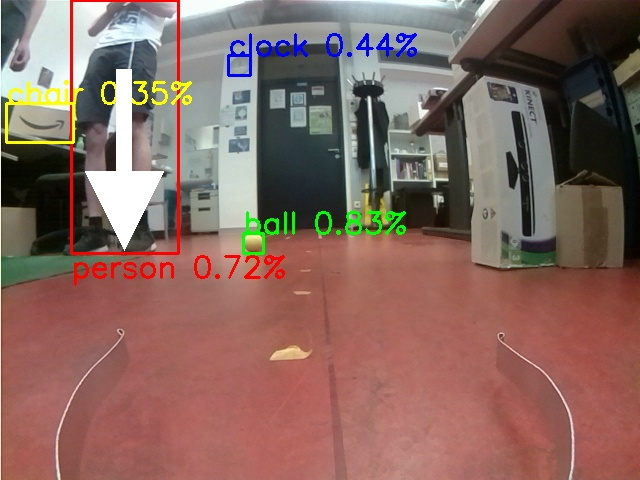
\includegraphics[width=\linewidth]{images/implementation/bounding_box_position}
\caption{The white arrow marks the relevant coordinates of the bounding box.}
\label{fig:bounding_box_position}
\end{figure}


All detected objects are published to the \enquote{\texttt{ball\_pos}} topic which is subscribed by the navigation node. The detections are published as a vector3 with \textit{x} being the percentage offset from the left side of the image of the \textit{x}-coordinate of the center of the detection, \textit{y} the percentage offset from the upper edge of the image to the lower border of the detection bounding box (\autoref{fig:bounding_box_position}) and \textit{z} the number of the detected class. The meaning of the percentage values for \textit{x} are 0.0 means left side of the image, 0.5 center and 1.0 right side. For the percentage values for \textit{y} 0.0 means top edge of the image, 0.5 center and 1.0 lower edge.

Additionally, opencv is used to render the detections on the original image with confidence and class name (\autoref{fig:detection_bounding_box_rendered}). Afterwards ist is converted back to an image message and published on \enquote{\texttt{debug\_image}} which is subscribed by the cockpit.

\section{Distance and position calculation}
\label{Distance and position calculation}
\subsection{Requirements}
In the next steps we have considered the position calculation of objects. A relatively accurate position would give us the possibility to approach objects relatively accurately and still not lose orientation in case of incorrect detection. In addition, delays can be calculated out.

For the implementation we wanted to use the incoming images. This would not require an additional sensor and we can continue to use the object recognition directly.

\subsection{Methods and failures}
For the implementation we tried several approaches. We distinguished between the \textit{x}-axis calculation and the \textit{y}-axis calculation. For simplification, we always considered the camera of the robot as the origin of the coordinate system and the objects outside changed their position with the movement of the robot. The \textit{y}-axis represented the right and left position of an object from the point of view of the robot. The \textit{x}-axis in turn represented the positive forward direction. Since we assume a flat floor and the robot cannot change the height, we see the Z-axis as irrelevant.

The units for the axes have been calculated in millimeters to simplify control.
For testing purposes, we took several pictures of the ball in several positions and
evaluated them with different methods.

\subsubsection{Horizon Approach}
The idea behind the approach is that nothing can exceed the horizon and thus there is a fixed scaling for the distance, which approaches the horizon asymptotically exponentially.
If the distance from the camera to the beginning of the image is known, this can be used to infer the distance to the object. For this you have to take the lowest position of the object and the relation of the position to the horizon. Then you can insert the relation into the function for the increasing distance which should be similar to this:

\begin{figure}[htbp]
\centering
\includesvg[width=\linewidth,inkscapelatex=false]{images/implementation/exponentialAsymptote.svg}
\caption{the y-axis gives us the distance and the
x-axis the position of the object between lense (0) and horizon(asymptote)}
\label{fig:exponentialAsymptoteGraph}
\end{figure}

The problem with the approach, however, was that the calculation depended heavily
on the distance from camera to image start and this was difficult to measure. In
addition, the results became inaccurate quite quickly, since the exponential change
with increasing distance also increased the inaccuracy exponentially.

\subsubsection{Focal-length Approach}
In this approach, we used the focal length and sensor size of the camera. Considering the real object and the projection, which is thrown through the lens onto the sensor, the rays allow to apply the intercept theorem. Distortions due to the lens were neglected for the time being. With the second intercept theorem you can conclude that the relation between the focal length of the camera and the size of the object on the sensor must be the same relation as the relation between the distance from the sensor to the object to the size of the object. Thus 3 constants
would be necessary, which must be known:
\begin{itemize}
\item Focal length sensor
\item Sensor size
\item Size of the object
\end{itemize}

Assuming that $f$ is the focal length of the camera in mm, $h_s$ the height of the object presented on the sensor in mm and $h_o$ the height of the object in the real world in mm, then the formula to calculate the distance in forward direction from the camera to the object is

\begin{align}
    x = \frac{f}{h_s} \cdot h_o
\end{align}

The size of the object on the sensor can be determined simply by the relative size of the object on the image in relation to the image itself multiplied by the sensor size.
The advantage of this procedure was that we got back quite exact values
independent of the camera height. Even at greater distances, the deviations were still manageable, which was more than sufficient for our scenario.
Disadvantage, however, was that we would thus be bound to fixed objects, since the size could no longer be changed.

\subsubsection{Relation Approach}
Here we try to determine the distance to the center of the image by the relative
position of the ball. For this again the size or width of the object is necessary as a relation. First we measure the width and the distance to the center of the detected box of the object. In the next step we look how many times the object fits into the distance to the center of the image. The amount will then be multiplied by the real world size of the object. The result will be the distance from the center to the object.

With this method, we have managed to obtain fairly accurate measurements, with
deviations of just about 3cm. More details on section below. Moreover, only one constant is necessary. Also disadvantage here again is that the size of the object must be known and therefore the object can be exchanged by another object only with difficulty.

\subsection{Result}
Since our camera is not always at the same position due to modifications and thus our first approach would no longer work and lead to large inaccuracies. 
On the other hand, the Focal Length and Relation Approach were the most suitable for our scenario. For our purposes we have chosen tennis balls, which are standardized by the ITF and have only slight variations in size \autocite{Int_TennisFederation}. In our case, we assumed a diameter of 6.7 cm. In order to test the procedures properly, we took several pictures from the robot, placing the ball at different positions and moving the camera vertically. As test positions we took:
\begin{itemize}
\item X: 20cm, Y: 0cm
\item X: 40cm, Y: 0cm
\item X: 60cm, Y: 0cm
\item X: 100cm, Y: 0cm
\item X: 100cm, Y: -20cm
\end{itemize}

For each image, we recorded the camera once in the lower anchorage of the robot and once in the upper anchorage of the robot. Since we use the rpi-wwcam2 the specifications were given by Prof. Dr. Ihme \autocite{Ihme_Latenzarme}. For the further sensor specifications informations like sensor size can also be found on the Internet, e.g. in the Reichelt e-shop \autocite{Reichelt_RPIWWCAM2}. However, the sensor size proves to be difficult, which is unfortunately specified in inches in most cases. For this, a table is needed to find out the height and width of the sensor, as provided by the website Photoreview.com \autocite{UnravellingSensor}. The following tables \autoref{table:positionCalculationHigh} and \autoref{table:positionCalculationLow} showing the results. For the X-Position the Focal Length Approach was used and for the Y-Position the Relation Approach.

\begin{table}[h]
  \caption{Results of position calculation with high camera.}
  \label{table:positionCalculationHigh}
  \renewcommand{\arraystretch}{1.2}
  \centering
  \sffamily
  \begin{footnotesize}
    \begin{tabularx}{0.58\linewidth}{l L L L L L L L}
      \toprule
      \textbf{Picture} & \textbf{X (in cm)} & \textbf{Y (in cm)} \\
      \midrule
        (20, 0)  & 23.47   & -1.71      \\
        (40, 0)  & 39.49   & -2.33      \\
        (60, 0)  & 56.89   & -2.1       \\
        (100, 0) & 90.72   & -2.8       \\
        (100, -20) & 95.91 & -21.34     \\
      \bottomrule
    \end{tabularx}
  \end{footnotesize}
  \rmfamily
\end{table}

\begin{table}[h]
  \caption{Results of position calculation with low camera.}
  \label{table:positionCalculationLow}
  \renewcommand{\arraystretch}{1.2}
  \centering
  \sffamily
  \begin{footnotesize}
    \begin{tabularx}{0.58\linewidth}{l L L L L L L L}
      \toprule
      \textbf{Picture} & \textbf{X (in cm)} & \textbf{Y (in cm)} \\
      \midrule
        (20, 0)    & 23.15  & -2.66        \\
        (40, 0)    & 38.58  & -0.8         \\
        (60, 0)    & 56.89  & -1.6         \\
        (100, 0)  & 88.34  & -1.76        \\
        (100, -20) & 98.73  & -22.86       \\
      \bottomrule
    \end{tabularx}
  \end{footnotesize}
  \rmfamily
\end{table}


Both tables show only minimal deviations of $\pm$3cm at the beginning. Only with further distance deviations of about 10cm resulted. In addition, the lens of the camera has a strong fisheye in the center, which would explain why the position (100, 0) has a much stronger deviation than the position (100, -20). However, the latter can be neglected in the deviation, since theoretically the position is always recalculated when approaching. For larger problems, however, the distortion can still be calculated using a checkerboard pattern.

The deviations were most likely also caused by measurement inaccuracies when measuring the ball and the distance measurements for the test images, since these were carried out in a room and with measurement materials that were not designed for this purpose.

Nevertheless, a complete implementation of both methods and thus a real test procedure was not achieved, because in addition to the exact position recognition, an extended navigation procedure is also necessary, which was not possible to implement due to time constraints.

\section{Conclusion}

Over the course of this project, we managed to create a system that is able to detect sports balls, maneuver towards them, collect them, detect the destination and bring the sports ball to the destination. To achieve this, we used a TurtleBot3 Burger as a mobile manipulation plattform in combination with \ac{ROS} and a docker container setup that allows for an easy reproduction and transfer of the system. We managed to find a fast and accurate object detection architecture that is able to process images at a fast enough pace that the detections can be used for navigating the TurtleBot. The system runs partially on the TurtleBot and partially on a laptop where the images are processed. This allowed for a faster processing of the images. We furthermore implemented a calculation of the distance from the camera to the detected objects based solely on the image received from the camera, although it was not used by the navigation in the end.

Although we ran into some problems regarding the technical setup and the communication between the TurtleBot and the laptop and the delay due to the distributed system, the final result managed to meet our expectations. The system is able to execute the desired tasks rather reliably. 

There are some areas left that could be looked further into in the future: The distance calculation could be used to steer the TurtleBot more precisely and change the speed depending on the distance from the target for smoother navigation. . Also, a detection model could be trained specifically for the desired tasks to enhance the detection behavior even more.

In the future an absolute position calculation as described in chapter \ref{Distance and position calculation} could be used to maneuver around obstacles. With this approach, positions could be recognized and remembered quite exactly. Problems like the object moving out of sight, delayed informations due to network problems or the object is not recognized all the time could be fixed by this.  However, it would be necessary to measure the robot's track while driving in order to update the positions of the surrounding objects if they are not recognizable. A dimension of the wheels and the rotational speed of the wheels would be one way to make this happen. In addition, an extended recognition of obstacles and driving around them would be possible. For this purpose, a self-trained neural network that is not limited to the given classes of the model used in this project would be advantageous.

The position detection can also be improved by calculating the distortion caused by the fisheye to avoid larger deviations in the center of the image. In addition, position recognition using \ac{AI} or multiple images from multiple perspectives instead of just one image would be conceivable in order to find calculate the position regardless of the size of the objects.

\section*{Acronyms}
\addcontentsline{toc}{section}{Acronyms}
\begin{acronym}[IEEE]
\acro{AI}{Artificial Intelligence}
\acro{CSPNet}{Cross Stage Partial Network}
\acro{mAP}{Mean Average Precision}
\acro{OS}{Operating System}
\acro{PANet}{Path Aggregation Network}
\acro{ROS}{Robot Operating System}
\acro{SSH}{Secure Shell}
\acro{SPP}{Spatial Pyramid Pooling}
\acro{TCP}{Transmission Control Protocol}
\acro{tty}{TeleTYpewriter (UNIX command)}
\acro{YOLO}{You Only Look Once}
\end{acronym}

\addcontentsline{toc}{section}{List of Tables}
\listoftables

\addcontentsline{toc}{section}{List of Figures}
\listoffigures

\addcontentsline{toc}{section}{List of Listings}
\lstlistoflistings

% Literaturverzeichnis
\addcontentsline{toc}{section}{Literature}
\printbibliography

\appendix
\section{Appendix}
\subsection{Code}

Code of the Docker Compose container setup:

{\scriptsize
\begin{lstlisting}[language=yaml,frame=single,caption=docker-compose.yml,label=code:compose]
services:
  roscore:
    image: ros:noetic-ros-core
    command: stdbuf -o L roscore
    tty: true
    stdin_open: true
    environment:
      ROS_IP: ${MASTER_IP}
    network_mode: host

  detect:
    build:
      context: ./docker
      dockerfile: Dockerfile
    command: /watchdog.sh detect.py
    tty: true
    stdin_open: true
    environment:
      ROS_MASTER_URI: http://${MASTER_IP}:11311
      ROS_IP: ${MASTER_IP}
    volumes:
      - ./detect:/app
    network_mode: host
    depends_on:
      - roscore

  nav:
    build:
      context: ./docker
      dockerfile: Dockerfile
    command: /watchdog.sh navigation.py
    tty: true
    stdin_open: true
    environment:
      ROS_MASTER_URI: http://${MASTER_IP}:11311
      ROS_IP: ${MASTER_IP}
    volumes:
      - ./navigation:/app
    network_mode: host
    depends_on:
      - roscore

  cockpit:
    build:
      context: ./docker
      dockerfile: Dockerfile
    command: /watchdog.sh cockpit.py
    tty: true
    stdin_open: true
    environment:
      ROS_MASTER_URI: http://${MASTER_IP}:11311
      ROS_IP: ${MASTER_IP}
    volumes:
      - ./cockpit:/app
    network_mode: host
    depends_on:
      - roscore
\end{lstlisting}
}

\subsection{Links}
\noindent
Code Repository on GitHub: \url{https://github.com/goseind/ball-schubser}.
\newline

\noindent
Demo Video on YouTube: \url{https://www.youtube.com/watch?v=InvO-HXr4YA}.

\end{document}
